% (c)~2012 Dimitrios Vrettos - d.vrettos@gmail.com
% (c) 2014 Daniele Zambelli - daniele.zambelli@gmail.com

\section{Esercizi}

\begin{comment}
\subsection{Esercizi dei singoli paragrafi}

%\subsubsection*{3.2 - Frazioni}
\subsubsection*{\numnameref{sec:03_frazioni}}

\begin{esercizio}
\label{ese:3.1}
Da un cartoncino rettangolare quadrettato di lati rispettivamente~5 unità 
e~8~unità viene ritagliata la forma colorata in grigio, come mostrato nella 
figura.
\begin{center}
 % (c) 2012 Dimitrios Vrettos - d.vrettos@gmail.com
% Esercizio 3.1

\begin{tikzpicture}
\draw[step=5mm, black] (0,0) grid (40mm,25mm);

\fill[gray, opacity=.4] (10mm,5mm) rectangle (15mm,10mm);
\fill[gray, opacity=.4] (25mm,5mm) rectangle (35mm,10mm);
\fill[gray, opacity=.4] (10mm,10mm) rectangle (30mm,15mm);
\fill[gray, opacity=.4] (5mm,15mm) rectangle (30mm,20mm);

\draw[|-|] (0,26.5mm) -- (40mm,26.5mm);
\node (8u) at (20mm,30mm) {$8\text{ unità}$};

\draw[|-|] (41.5mm,0) -- (41.5mm,25mm);
\node[rotate=-90] (5u) at (45mm,12.5mm) {$5\text{ unità}$};
\end{tikzpicture}

\end{center}
Quale delle seguenti espressioni ti sembra più corretta per esprimere la 
relazione tra il cartoncino e la forma ritagliata?
\begin{enumeratea}
 \item La forma ottenuta è più piccola del cartoncino;
 \item la forma ottenuta è un poligono con un numero maggiore di lati rispetto 
 al cartoncino dato;  
 \item la forma ottenuta rappresenta i~12/40 del cartoncino.
\end{enumeratea}
Sbaglio se affermo che la parte colorata è i~$3/10$ del cartoncino?
\end{esercizio}

\begin{esercizio}
\label{ese:3.2}
Il monte-premi di una lotteria è di \officialeuro\ 50\,000. 
Il primo premio è di \officialeuro\ 25\,000, 
il secondo di \officialeuro\ 10\,000, 
il terzo di \officialeuro\ 5\,000, 
il quarto di \officialeuro\ 4\,000, 
il quinto e il sesto premio sono uguali.
Nella figura un quadretto rappresenta \officialeuro\ 1\,000.
\begin{center}
 % (c) 2012 Dimitrios Vrettos - d.vrettos@gmail.com
% Esercizio 3.2
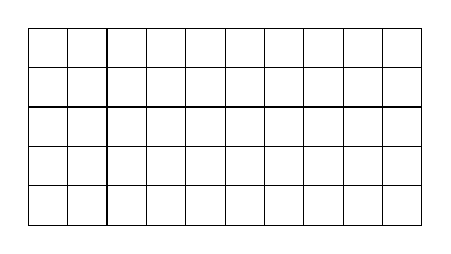
\begin{tikzpicture}
\draw[step=5mm, black] (0,0) grid (50mm,25mm);
\end{tikzpicture}

\end{center}
\begin{enumeratea}
 \item Colora con colori diversi i quadretti quanti servono per rappresentare 
 i sei premi, un colore per ogni premio;
 \item quale parte del monte-premi è stata incassata da chi ha vinto 
 il secondo premio? Esprimi questa parte con una frazione;
 \item Marco ha vinto il sesto premio: quanto ha vinto?
\end{enumeratea}
\end{esercizio}

\begin{esercizio}
 \label{ese:3.3}
La figura seguente è composta da~11 quadratini, alcuni bianchi altri grigi.
\begin{center}
 % (c) 2012 Dimitrios Vrettos - d.vrettos@gmail.com
% Esercizio 3.3
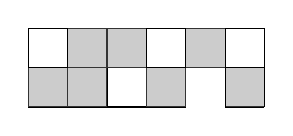
\begin{tikzpicture}
  \begin{scope}[step=5mm, black]
    \draw (0,0) grid (20mm,10mm);
    \draw (20mm,5mm) grid (25mm,10mm);
    \draw (25mm,0) grid (30mm,10mm);
  \end{scope}
  \begin{scope}[gray, opacity=.4]
    \fill (0,0) rectangle (10mm,5mm);
    \fill (15mm,0) rectangle (20mm,5mm);
    \fill (25mm,0) rectangle (30mm,5mm);
    \fill (5mm,5mm) rectangle (15mm,10mm);
    \fill (20mm,5mm) rectangle (25mm,10mm);   
  \end{scope}
  \draw (25mm,0)--(25mm,5mm);
\end{tikzpicture}

\end{center}
\emph{Completa}: la figura è divisa in due parti mediante la colorazione: 
la parte grigia
rappresenta \ldots\ldots\ldots dell'intera figura, mentre la parte bianca 
ne è \ldots\ldots\ldots
\end{esercizio}

\begin{esercizio}
 \label{ese:3.4}
 Di ciascuna figura colora la parte indicata dalla frazione.
\begin{center}
 % (c) 2012 Dimitrios Vrettos - d.vrettos@gmail.com
% Esercizio 3.4

\begin{tikzpicture}

\draw  (0,0) circle(.8cm);
\draw (1.8cm,-.8cm) rectangle (4.1cm,.8cm);
\node [star, star point height=.5cm, minimum size=1.8cm, rotate=45, draw] at (5.9cm,0) {};

\node (cercio) at (0,1.5cm) {$\displaystyle\frac{3}{5}$};
\node (rettangolo) at (2.95cm,1.5cm) {$\displaystyle\frac{2}{3}$};
\node (cercio) at (5.9cm,1.5cm) {$\displaystyle\frac{1}{2}$};
\end{tikzpicture}

\end{center}
\end{esercizio}

\begin{esercizio}
\label{ese:3.5}
 Indica se le frazioni sono proprie (P), improprie (I) o apparenti (A).
 \begin{multicols}{3}
 \TabPositions{0.6cm}
 \begin{enumeratea}
 \item $\dfrac{3}{4}$ \tab\quad\boxP\quad\boxI\quad\boxA\vspace{1.1ex}
 \item $\dfrac{8}{3}$ \tab\quad\boxP\quad\boxI\quad\boxA
 \item $\dfrac{12}{3}$ \tab\quad\boxP\quad\boxI\quad\boxA\vspace{1.1ex}
 \item $\dfrac{5}{2}$ \tab\quad\boxP\quad\boxI\quad\boxA
 \item $\dfrac{5}{3}$ \tab\quad\boxP\quad\boxI\quad\boxA\vspace{1.1ex}
 \item $\dfrac{3}{2}$ \tab\quad\boxP\quad\boxI\quad\boxA
 \end{enumeratea}
 \end{multicols}
\end{esercizio}

\begin{esercizio}
\label{ese:3.6}
Trova le frazioni equivalenti completando.
 \begin{multicols}{4}
 \begin{enumeratea}
 	\item $\dfrac{3}{4}=\dfrac{\ldots}{12}$
 	\item $\dfrac{12}{16}=\dfrac{3}{\ldots}$
 	\item $\dfrac{5}{2}=\dfrac{\ldots}{10}$
 	\item $\dfrac{21}{35}=\dfrac{\ldots}{5}$
 \end{enumeratea}
 \end{multicols}
\end{esercizio}

\begin{esercizio}
 \label{ese:3.7}
 Indica almeno tre frazioni equivalenti a ciascuna delle seguenti.
 \begin{multicols}{6}
 \begin{enumeratea}
 	\item $\dfrac{5}{6}$
 	\item $\dfrac{3}{5}$
 	\item $\dfrac{12}{60}$
 	\item $\dfrac{2}{3}$
 	\item $\dfrac{1}{2}$
 	\item $\dfrac{5}{2}$
 \end{enumeratea}
 \end{multicols}
\end{esercizio}

\begin{esercizio}
 \label{ese:3.8}
Nella figura che segue il quadratino colorato rappresenta~$1/4$ del quadrato 
grande; costruisci una figura che rappresenti~$8/4$ del quadrato grande 
accostando opportunamente altri quadrati uguali.
 \begin{center}
 % (c) 2012 Dimitrios Vrettos - d.vrettos@gmail.com
% Quadrato 1/4
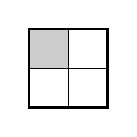
\begin{tikzpicture}
  \begin{scope}[scale=1,every node/.style={minimum size=5mm}]
    \draw[step=5mm, black] (0,0) grid (1,1);
    \fill[gray, opacity=.4] (0,.5) rectangle (.5,1);
    \draw[black,thick] (0,0) rectangle (1,1);
  \end{scope} 
\end{tikzpicture}

 \end{center}
\end{esercizio}

\begin{esercizio}
 \label{ese:3.9}
Riduci ai minimi termini le seguenti frazioni.
 \begin{multicols}{6}
 \begin{enumeratea}
 \item $\dfrac{4}{6}$\vspace{1.1ex}
 \item $\dfrac{8}{2}$\vspace{1.1ex}
 \item $\dfrac{2}{10}$
 \item $\dfrac{18}{16}$\vspace{1.1ex}
 \item $\dfrac{3}{12}$\vspace{1.1ex}
 \item $\dfrac{6}{20}$
 \item $\dfrac{80}{100}$\vspace{1.1ex}
 \item $\dfrac{8}{12}$\vspace{1.1ex}
 \item $\dfrac{9}{6}$
 \item $\dfrac{10}{15}$\vspace{1.1ex}
 \item $\dfrac{14}{49}$\vspace{1.1ex}
 \item $\dfrac{15}{21}$
 \item $\dfrac{16}{6}$\vspace{1.1ex}
 \item $\dfrac{18}{15}$\vspace{1.1ex}
 \item $\dfrac{20}{12}$
 \item $\dfrac{21}{9}$\vspace{1.1ex}
 \item $\dfrac{24}{30}$\vspace{1.1ex}
 \item $\dfrac{25}{15}$
 \end{enumeratea}
 \end{multicols}
\end{esercizio}

\end{comment}

\begin{esercizio}
 \label{ese:3.10}
Riduci ai minimi termini le seguenti frazioni.
 \begin{multicols}{6}
 \begin{enumeratea}
 \item $\dfrac{27}{21}$\vspace{1.1ex}
 \item $\dfrac{28}{14}$\vspace{1.1ex}
 \item $\dfrac{30}{16}$
 \item $\dfrac{32}{24}$\vspace{1.1ex}
 \item $\dfrac{35}{10}$\vspace{1.1ex}
 \item $\dfrac{36}{81}$
 \item $\dfrac{40}{6}$\vspace{1.1ex}
 \item $\dfrac{42}{21}$\vspace{1.1ex}
 \item $\dfrac{45}{27}$
 \item $\dfrac{48}{60}$\vspace{1.1ex}
 \item $\dfrac{12}{30}$\vspace{1.1ex}
 \item $\dfrac{135}{77}$
 \item $\dfrac{121}{22}$\vspace{1.1ex}
 \item $\dfrac{87}{99}$\vspace{1.1ex}
 \item $\dfrac{15}{360}$
 \item $\dfrac{110}{30}$\vspace{1.1ex}
 \item $\dfrac{240}{75}$\vspace{1.1ex}
 \item $\dfrac{140}{294}$
 \end{enumeratea}
 \end{multicols}
\end{esercizio}

\begin{comment}
\begin{inaccessibleblock}[Figura: TODO]
 \begin{figure}[t]
 \begin{minipage}[b]{.45\textwidth}
 \centering% (c) 2012 Dimitrios Vrettos - d.vrettos@gmail.com
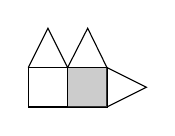
\begin{tikzpicture}
\draw (0,0) rectangle  (10mm,5mm);
\draw (0,5mm) -- (2.5mm,10mm)--(5mm,5mm)--(7.55mm,10mm)--(10mm,5mm);
\draw (10mm,5mm) -- (15mm,2.5mm)--(10mm,0);
\draw (5mm,0) -- (5mm,5mm);

\fill[gray, opacity=.4](5mm,0) rectangle  (10mm,5mm);
\end{tikzpicture}

 \caption{Esercizio~\ref{ese:3.11}}\label{fig:3.4}
 \end{minipage}\hfil
\begin{minipage}[b]{.45\textwidth}
 \centering% (c) 2012 Dimitrios Vrettos - d.vrettos@gmail.com
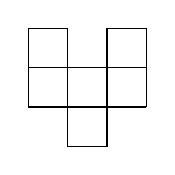
\begin{tikzpicture}
\draw[step=5mm] (0,0) grid  (15mm,5mm);
\draw (0,5mm) rectangle  (5mm,10mm);
\draw (10mm,5mm) rectangle  (15mm,10mm);
\draw (5mm,0) rectangle  (10mm,-5mm);
\end{tikzpicture}

 \caption{Esercizio~\ref{ese:3.12}}\label{fig:3.5}
 \end{minipage}
\end{figure}
\end{inaccessibleblock}

\begin{esercizio}
 \label{ese:3.11}
Si può dire che la parte colorata in grigio della figura corrisponde 
a~$\frac{1}{5}$ della figura stessa?
\end{esercizio}

\begin{esercizio}
 \label{ese:3.12}
Costruisci una figura che corrisponde a~$\frac{11}{6}$ della figura seguente.
\end{esercizio}

\begin{esercizio}
 \label{ese:3.13}
Per ciascuno dei seguenti disegni la parte colorata in grigio rappresenta 
sempre la frazione~$\dfrac{3}{4}$ del quadrato bianco?
 \begin{center}
 % (c) 2012 Dimitrios Vrettos - d.vrettos@gmail.com
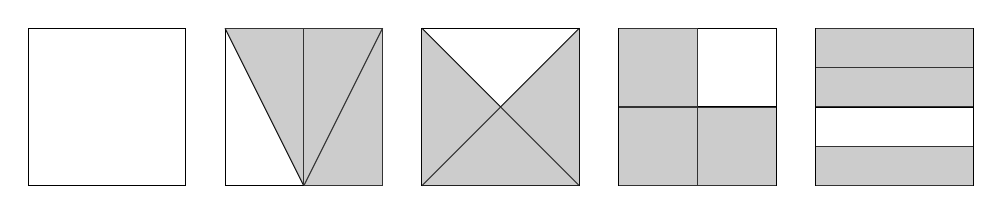
\begin{tikzpicture}
  \begin{scope}[x=25mm,y=5mm]
    % Costruzione dei 5 quadrati
    \foreach \x in {0,1,...,4}
      \node[draw, minimum size=20mm](quad) at(\x,0) {};
    %  Nomi
%     \foreach \c [count=\x from 0] in {$A$,$B$,$C$,$D$,$E$} 
%       \node[below=13mm] at (\x,0) {\c};
    %  quadrato B
    \draw(15mm,2)--(1,-2);
    \draw(1,-2)--(35mm,2);
    \draw(1,-2)--(1,2);
    \begin{scope}[fill=gray, fill opacity=.4]
      \fill (15mm,2)--(1,2)--(1,-2);
      \fill (1,-2) rectangle (35mm,2);
    \end{scope}
    % quadrato C
    \draw(40mm,2)--(60mm,-2);
    \draw (40mm,-2) -- (60mm,2);
    \begin{scope}[fill=gray, fill opacity=.4]
      \fill (40mm,2)--(60mm,-2)--(40mm,-2);
      \fill (60mm,2)--(60mm,-2)--(2,0);
    \end{scope}
    % quadrato D
    \draw (65mm,0) -- (85mm,0);
    \draw (3,-2) -- (3,2);
    \begin{scope}[fill=gray, fill opacity=.4]
      \fill (65mm,-2) rectangle (3,2);
      \fill (3,-2) rectangle (85mm,0);
    \end{scope}
    % quadrato E
    \foreach \y in {-1,0,1}
      \draw (90mm,\y) -- (110mm,\y);
    \begin{scope}[fill=gray, fill opacity=.4]
      \fill (90mm,2) rectangle (110mm,0);
      \fill (90mm,-2) rectangle (110mm,-1);
    \end{scope}
  \end{scope}
\end{tikzpicture}

 \end{center}
\end{esercizio}

\begin{esercizio}
 \label{ese:3.14}
Il segmento nel disegno rappresenta i~$3/5$ dell'intero.
 \begin{center}
 % (c) 2012 Dimitrios Vrettos - d.vrettos@gmail.com
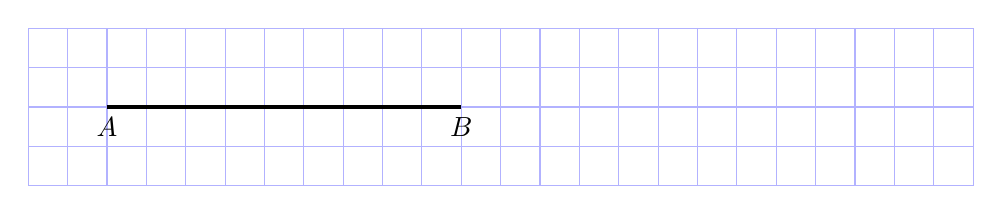
\begin{tikzpicture}
\draw[step=5mm, blue, opacity=.3](0,0) grid (120mm,20mm);
\draw[very thick](10mm,10mm) node [below] {$A$} --(55mm,10mm) node [below] {$B$};
\end{tikzpicture}

 \end{center}
Ti basta questa informazione per costruire l'intero? Come procederesti?
\end{esercizio}

\begin{esercizio}
 \label{ese:3.15}
Disegna un segmento come grandezza unitaria e dimostra che la frazione~$3/5$ 
è equivalente a~$6/10$ ma non a~$9/25$
% \begin{center}
% % (c) 2012 Dimitrios Vrettos - d.vrettos@gmail.com
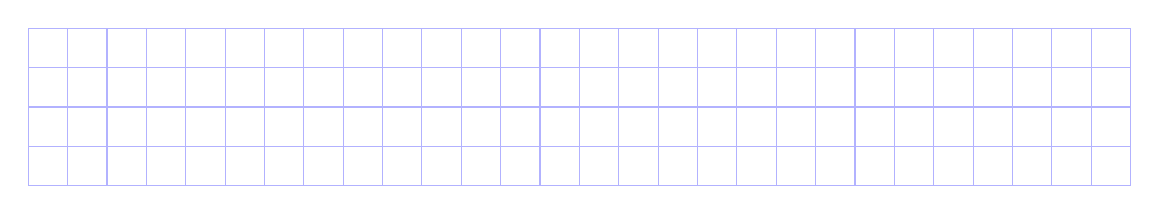
\begin{tikzpicture}
\draw[step=5mm, blue, opacity=.3](0,0) grid (140mm,20mm);
\end{tikzpicture}

% \end{center}
\end{esercizio}

\begin{esercizio}
 \label{ese:3.16}
Usando una grandezza unitaria arbitraria, stabilisci quale delle seguenti 
frazioni rappresenta l'intero e quale un suo multiplo:
\[\dfrac{2}{4}\qquad\dfrac{6}{3}\qquad\dfrac{5}{5}\qquad\dfrac{8}{4}\qquad
\dfrac{9}{4}.\]
\end{esercizio}

\end{comment}
%%%%%%%%%%%%%%%%%%%%%%%%%%%%%%%%%%%%%%%%%%%%
%~3.3 Dalle frazioni ai numeri razionali %
%%%%%%%%%%%%%%%%%%%%%%%%%%%%%%%%%%%%%%%%%%%%
%\subsubsection*{3.3 - Dalle frazioni ai numeri razionali}
\subsubsection*{\numnameref{sec:03_razionali}}

\begin{esercizio}
 \label{ese:3.17}
Raggruppa le seguenti frazioni in insiemi di frazioni equivalenti.
Etichetta l'insieme con un numero razionale, prendendo per ogni gruppo la 
frazione ridotta ai minimi termini.

\[\frac{1}{3};\,\frac{2}{4};\,-\frac{5}{2};\,\frac{6}{-14};\,\frac{-12}{4};\,
\frac{3}{6};\,\frac{-3}{-9};\,
\frac{10}{-4};\,\frac{10}{20};\,\frac{-18}{42};\,\frac{5}{15};\,
-\frac{9}{21};\,-\frac{15}{6};\,\frac{4}{12}.\]
\end{esercizio}

\begin{esercizio}
 \label{ese:3.18}
 Riscrivi le seguenti frazioni improprie come somma di un numero naturale e 
 una frazione propria.
\[\frac{10}{3};\,\frac{17}{9};\,\frac{11}{2};\,\frac{25}{3};\,\frac{17}{10};\,
\frac{15}{6}.\]
\end{esercizio}

%\subsubsection*{3.4 - La scrittura dei numeri razionali}
\subsubsection*{\numnameref{sec:03_decimali}}

\begin{esercizio}
 \label{ese:3.19}
 Senza eseguire le divisioni indica quali di queste frazioni possono essere 
 scritte come numero decimale finito (DF), quali come numero decimale 
 periodico (DP) e quali come numero intero (I):
 
 \begin{multicols}{2}
 \TabPositions{1cm}
 \begin{enumeratea}
% 	\spazielenx
 \item $-\dfrac{3}{2}$ 
\tab\qquad\boxDF\qquad\boxDP\quad\enspace\enspace\boxI\vspace{1.1ex}
 \item $-\dfrac{6}{5}$ 
\tab\qquad\boxDF\qquad\boxDP\quad\enspace\enspace\boxI\vspace{1.1ex}
 \item $\dfrac{2}{25}$ 
\tab\qquad\boxDF\qquad\boxDP\quad\enspace\enspace\boxI\vspace{1.1ex}
 \item $\dfrac{5}{8}$ \tab\qquad\boxDF\qquad\boxDP\quad\enspace\enspace\boxI
 \item $\dfrac{5}{6}$ 
\tab\qquad\boxDF\qquad\boxDP\quad\enspace\enspace\boxI\vspace{1.1ex}
 \item $-\dfrac{5}{12}$ 
\tab\qquad\boxDF\qquad\boxDP\quad\enspace\enspace\boxI\vspace{1.1ex}
 \item $\dfrac{12}{6}$ 
\tab\qquad\boxDF\qquad\boxDP\quad\enspace\enspace\boxI\vspace{1.1ex}
 \item $\dfrac{5}{10}$ \tab\qquad\boxDF\qquad\boxDP\quad\enspace\enspace\boxI
 \end{enumeratea}
 \end{multicols}
\end{esercizio}

\begin{esercizio}
\label{ese:3.20}
Trasforma le seguenti frazioni in numeri decimali.
\begin{multicols}{6}
\begin{enumeratea}
\spazielenx
\item $\dfrac{13}{2}$
\item $\dfrac{11}{3}$
\item $\dfrac{3}{5}$
\item $\dfrac{15}{6}$
\item $\dfrac{17}{7}$
\item $\dfrac{15}{8}$
\item $\dfrac{12}{9}$
\item $\dfrac{127}{10}$
\item $\dfrac{122}{11}$
\item $\dfrac{13}{12}$
\item $\dfrac{35}{121}$
\item $\dfrac{121}{35}$
\item $\dfrac{12}{10}$
\item $\dfrac{127}{100}$
\item $\dfrac{122}{1100}$
\item $\dfrac{13}{100}$
\item $\dfrac{35}{1000}$
\item $\dfrac{121}{10000}$
\item $\dfrac{12}{5}$
\item $\dfrac{13}{7}$
\item $\dfrac{15}{4}$
\item $\dfrac{5}{8}$
\item $\dfrac{32}{9}$
\item $\dfrac{21}{20}$
\item $\dfrac{37}{18}$
\item $\dfrac{2}{21}$
\end{enumeratea}
\end{multicols}
\end{esercizio}

\begin{esercizio}[\Ast]
\label{ese:3.21}
Trasforma in frazioni i seguenti numeri decimali.
\begin{multicols}{4}
\begin{enumeratea}
 \item 12,5
 \item 4,2
 \item 6,25
 \item 3,75
 \item 0,1
 \item 2,5
 \item 100,100
 \item 0,12
 \item 1,1030
 \item 0,00100
 \item 100,0010
 \item 0,0001
 \item 1,25
 \item 0,08
 \item 1,002
 \item 15,675
 \item 1,7
 \item 1,46
 \item 0,13
 \item 0,149
 \item 5,015
 \item 3,21
 \item 2,3
 \item 1,086
\end{enumeratea}
\end{multicols}
\(\left[a)~\frac{25}{2},\quad b)~\frac{21}{5}\quad c)~\frac{25}{4}\quad 
d)~\frac{15}{4}\quad e)~\frac{1}{10}\quad f)~\frac{5}{2} \dots \right]\)
\end{esercizio}


\begin{comment}
\begin{esercizio}
 \label{ese:3.22}
Completa la tabella.

 \begin{tabular*}{.9\textwidth}{@{\extracolsep{\fill}}*{6}{lccccc}}
 \toprule
 &\multicolumn{2}{c}{Parte}& & &\\
 Numero decimale & intera & decimale & Periodo & Antiperiodo & Frazione\\
 \midrule
 1,7521& & & & &\\
~$3,\overline{75}$& & & & &\\
~$12,1\overline{24}$& & & & &\\
~$1,0\overline{5}~$& & & & &\\
~$0,13\overline{57}~$& & & & &\\
 \bottomrule
 \end{tabular*}
\end{esercizio}

\end{comment}

% \clearpage
\begin{esercizio}
\label{ese:3.23}
 Trasforma i seguenti numeri decimali in frazioni.
\begin{multicols}{4}
\begin{enumeratea}
\item $-1,25$
\item 0,03;
\item $-2,\overline{1}$
\item $0,\overline{13}$
\item 5,080;
\item $3,7\overline{52}$
\item $-0,38$
\item $11,\overline{175}$
\item $0,01\overline{02}$
\item $0,12\overline{345}$
\item $100,\overline{100}$
\item $100,\overline{001}$
\item 0,08;
\item 0,2;
\item 0,1;
\item 0,03;
\item $23,\overline{5}$
\item $22,\overline{32}$
\item 0,25;
\item $31,\overline{02}$
\item $0,\overline{21}$
\item $2,3\overline{4}$
\item $3,21\overline{8}$
\item $0,03\overline{4}$
\end{enumeratea}
\end{multicols}
\end{esercizio}

\begin{esercizio}
\label{ese:3.24}
Scrivi la frazione generatrice di~$12,3\overline{45}$ 
Qual è la~614-esima cifra decimale del numero?
\end{esercizio}

\begin{esercizio}
\label{ese:3.25}
Calcola~$0,\overline{9}-3,\overline{9}$ Cosa osservi?
\end{esercizio}

%\subsubsection*{3.5 - I numeri razionali e la retta}
\subsubsection*{\numnameref{sec:03_retta}}

\begin{esercizio}
 \label{ese:3.26}
Rappresenta su una retta orientata, dopo aver scelto una opportuna unità di 
misura, i seguenti gruppi di numeri razionali, ciascun gruppo su una retta.

 \begin{enumeratea}
\spazielenx
 \item 
$\displaystyle{\frac{2}{3},\quad-\frac{3}{4},\quad\frac{5}{2},\quad-\frac{7}{12}
,\quad\frac{3}{2},\quad%
-\frac{11}{6},\quad\frac{9}{4}}$
 \item 
$\displaystyle{\frac{0}{4},\quad\frac{5}{4},\quad\frac{9}{4},\quad\frac{1}{2},
\quad\frac{19}{8},\quad\frac{3}{2}%
,\quad\frac{7}{4},\quad\frac{4}{2}}$
 \item 
$\displaystyle{\frac{10}{3},\quad\frac{5}{3},\quad~2,\quad\frac{0}{3},\quad\frac
{4}{3},\quad\frac{2}{3}%
,\quad\frac{5}{6},\quad\frac{13}{6}}$
 \item 
$\displaystyle{\frac{1}{2},\quad\frac{3}{4},\quad-\frac{5}{4},\quad-\frac{1}{2},
\quad\frac{7}{8},%
\quad-\frac{5}{16}}$
\item 
$\displaystyle{\frac{8}{5},\quad\frac{1}{2},\quad\frac{3}{10},\quad-\frac{7}{4},
\quad-\frac{3}{5}%
,\quad-\frac{11}{10}}$
 \end{enumeratea}
\end{esercizio}

\begin{esercizio}
 \label{ese:3.27}
 Scrivi i numeri razionali rappresentati dai punti segnati sulla retta nella 
 figura.
\begin{center}
% (c) 2012 Dimitrios Vrettos - d.vrettos@gmail.com
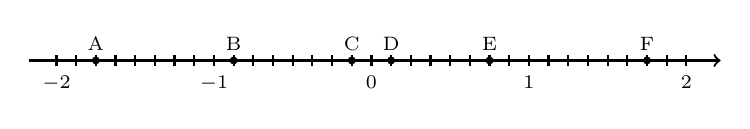
\begin{tikzpicture}
\begin{scope}[thick,font=\scriptsize]
\draw[->] (-10pt,0) -- (240pt,0);
  \foreach \x/\xtext in {%
      0/-2,.25/,.5/,.75/,
1/,1.25/,1.5/,1.75/,2/-1,2.25/,2.5/,2.75/,3/,%
      3.25/,3.5/,3.75/,4/0,4.25/,4.5/,4.75/,%
      5/,5.25/,5.5/,5.75/,6/1,6.25/,6.5/,6.75/,7/,7.25/,7.5/,7.75/,8/2}
    \draw[shift={(\x,0)}] (0pt,2pt) -- (0pt,-2pt) node[below] {$\xtext$};
\foreach \y/\ytext in {.5/$A$,2.25/$B$,3.75/$C$,4.25/$D$,5.5/$E$,7.5/$F$}
	 \draw[shift={(\y,0)}] (0pt,2pt) -- (0pt,-2pt) node[above=2pt] {$\ytext$};
\draw (.5,0) circle (1pt);
\draw (2.25,0) circle (1pt);
\draw (3.75,0) circle (1pt);
\draw (4.25,0) circle (1pt);
\draw (5.5,0) circle (1pt);
\draw (7.5,0) circle (1pt);
\end{scope}
\end{tikzpicture}

\end{center}

\end{esercizio}

\begin{esercizio}
 \label{ese:3.28}
Disegna su una retta orientata i seguenti numeri decimali, ciascun gruppo su 
una retta.
\begin{enumeratea}
 \item $0,6\qquad2,3\qquad-1,2\qquad-0,06$
 \item $+1,4\qquad-0,3\qquad-1,5\qquad0,2$
 \item $-0,8\qquad-1,6\qquad+4,91\qquad-1,17$
 \item $1,55\qquad2,01\qquad-3,0\qquad-2,10$
\end{enumeratea}
\end{esercizio}

%\subsubsection*{3.6 - Confronto tra numeri razionali}
\subsubsection*{\numnameref{sec:03_confronto}}

\begin{esercizio}
 \label{ese:3.29}
Inserisci tra le seguenti coppie di numeri razionali i simboli di 
maggiore~($>$), minore~($<$) o uguale~($=$).
\begin{multicols}{3}
\begin{enumeratea}
\spazielenx
 \item $\dfrac{4}{5}\,\ldots\,\dfrac{5}{7}$
 \item $-\dfrac{9}{5}\,\ldots\,-\dfrac{8}{3}$
 \item $-1\,\ldots\,\dfrac{1}{12}$
 \item $\dfrac{2}{7}\,\ldots\,\dfrac{6}{21}$
 \item $-\dfrac{1}{2}\,\ldots\,-\dfrac{3}{4}$
 \item $\dfrac{3}{5}\,\ldots\,\dfrac{6}{9}$
\end{enumeratea}
\end{multicols}
\end{esercizio}

\begin{esercizio}
 \label{ese:3.30}
Quale dei seguenti numeri razionali è il maggiore?

\[\frac{2}{3} \qquad \frac{3}{4} \qquad \frac{5}{8} \qquad \frac{3}{5},
\qquad\frac{7}{12}.\]
\end{esercizio}


\begin{esercizio}
 \label{ese:3.31}
Quale dei seguenti numeri razionali è il minore?

\[-\frac{2}{3} \qquad -\frac{3}{4} \qquad -\frac{5}{6} \qquad -\frac{1}{2},
\qquad-\frac{2}{5}.\]
\end{esercizio}

\begin{esercizio}
 \label{ese:3.32}
Scrivi in ordine crescente (dal più piccolo al più grande).

\[-\frac{2}{3} \qquad \frac{3}{4} \qquad -\frac{5}{6} \qquad \frac{1}{2},
\qquad-1 \qquad -\frac{2}{5} \qquad 0.\]
\end{esercizio}

\begin{esercizio}
 \label{ese:3.33}
Scrivi in ordine decrescente (dal più grande al più piccolo).

\[-\frac{3}{2} \qquad \frac{4}{3} \qquad -\frac{6}{5} \qquad \frac{2}{5},
\qquad-1 \qquad \frac{5}{2} \qquad 0\]
\end{esercizio}

 \begin{esercizio}
\label{ese:3.34}
Qual è la minore delle seguenti frazioni?
\[\boxA\quad\frac{2}{3}\qquad
\boxB\quad\frac{2}{7}\qquad
\boxC\quad\frac{3}{2}\qquad
\boxD\quad\frac{1}{2}.\]
\end{esercizio}

\begin{esercizio}
\label{ese:3.35}
Metti in ordine le seguenti frazioni.
\[\frac{3}{4};\qquad\frac{4}{3};\qquad\frac{11}{12};\qquad\frac{5}{3}.\]
\end{esercizio}

\begin{esercizio}
 \label{ese:3.36}
Ordina dal più piccolo al più grande.
\begin{enumeratea}
\item 10,011\qquad10,110\qquad11,001\qquad11,100;
\item 10,01\qquad11,11\qquad10,101\qquad10,001;
\item 0,101\qquad0,011\qquad0,110\qquad0,0101;
\item 1,0101\qquad1,1001\qquad1,0011\qquad1,0110;
\end{enumeratea}
\end{esercizio}

\begin{esercizio}
\label{ese:3.37}
Scrivi una frazione molto vicina a~$-\frac{2}{9}.$
\end{esercizio}

\begin{esercizio}
\label{ese:3.38}
Scrivi una frazione compresa tra:
\begin{multicols}{3}
\begin{enumeratea}
\item $\dfrac{3}{5}$ e~$\dfrac{7}{10}$
\item $\dfrac{5}{3}$ e~$\dfrac{1}{7}$
\item $\dfrac{1}{2}$ e~$\dfrac{2}{3}$
\end{enumeratea}
\end{multicols}
\end{esercizio}

\begin{esercizio}
\label{ese:3.39}
Quali disuguaglianze sono vere?
\begin{multicols}{2}
\TabPositions{2.5cm}
\begin{enumeratea}
\spazielenx
 \item $-\dfrac{7}{6}<-\dfrac{6}{7}$\tab\boxV\qquad\boxF
 \item $-\dfrac{7}{6}>+\dfrac{6}{7}$\tab\boxV\qquad\boxF
 \item $-\dfrac{7}{6}<+\dfrac{6}{7}$\tab\boxV\qquad\boxF
 \item $+\dfrac{7}{6}<-\dfrac{6}{7}$\tab\boxV\qquad\boxF
 \item $+\dfrac{7}{6}<+\dfrac{6}{7}$\tab\boxV\qquad\boxF
 \item $+\dfrac{7}{6}>-\dfrac{6}{7}$\tab\boxV\qquad\boxF
 \end{enumeratea}
\end{multicols}
\end{esercizio}

\begin{esercizio}
\label{ese:3.40}
Quale dei seguenti numeri è più vicino a~1?
\[\boxA\quad0,10\qquad\boxB\quad0,99\qquad\boxC\quad0,01\qquad\boxD\quad0,90\]
\end{esercizio}

 \begin{esercizio}
\label{ese:3.41}
Quale dei seguenti numeri è più vicino alla frazione~$\frac{1}{10}$?
\[\boxA\quad0,01\qquad\boxB\quad0,90\qquad\boxC\quad1,01\qquad\boxD\quad0,19\]
 \end{esercizio}

\begin{esercizio}
\label{ese:3.42}
Scrivi due numeri compresi tra:
\begin{multicols}{3}
\begin{enumeratea}
 \item 2,3 e 3,4;
 \item 3,4 e 3,6;
 \item $2,\overline{3}$ e~$2,\overline{4}$
 \item $1,1\overline{3}$ e~$1,2\overline{3}$
 \item $3,\overline{4}$ e~$3,\overline{6}$
 \item $1,\overline{35}$ e~$1,\overline{36}$
\end{enumeratea}
\end{multicols}
\end{esercizio}

\begin{esercizio}
 \label{ese:3.43}
Rappresenta su una opportuna retta numerica le seguenti frazioni e poi 
riscrivile in ordine crescente:
\[\frac{3}{4}; \quad \frac{3}{8}; \quad \frac{1}{3}; \quad \frac{5}{4}; 
\quad \frac{2}{5}; \quad \frac{6}{3}; \quad \frac{5}{6}; 
\quad \frac{12}{4}; \quad \frac{19}{8}; \quad \frac{16}{5}.\]
\end{esercizio}

%%%%%%%%%%%%%%%%%%%%%%%%%%%%%%%%%%%%%%%%%%%%%%%%%%%%%%%%%%%

\subsubsection*{\numnameref{sec:03_operazioni}}

\begin{esercizio}
 \label{ese:3.44}
Calcola le seguenti somme algebriche tra frazioni.
\begin{multicols}{4}
\begin{enumeratea}
\spazielenx
\item $\dfrac{1}{2} + \frac{3}{2}$
\item $\dfrac{7}{11} + \frac{4}{11}$
\item $\dfrac{3}{2} - \frac{5}{2}$
\item $\dfrac{8}{18} + \frac{5}{9}$
\item $\dfrac{6}{5} +~0$
\item $-\dfrac{3}{2}+\dfrac{4}{3}$
\item $-\dfrac{2}{3}+\dfrac{3}{4}$
\item $\dfrac{4}{3}-\dfrac{6}{5}$
\item $\dfrac{2}{5}+\dfrac{5}{8}$
\item $\dfrac{5}{8}+\dfrac{5}{6}$
\item $\dfrac{5}{6}-\dfrac{5}{12}$
\item $1-\dfrac{3}{2}$
\item $\dfrac{11}{5}+5$
\item $\dfrac{7}{3}-\dfrac{6}{4}$
\item $3-\dfrac{2}{3}$
\item $\dfrac{1}{5}-1$
\item $4+\dfrac{3}{2}-\dfrac{3}{4}$
\item $\dfrac{4}{3}+3-\dfrac{1}{2}$
\item $\dfrac{3}{4}+\dfrac{1}{4}-\dfrac{5}{4}$
\item $1-\dfrac{1}{2}+\dfrac{1}{3}-\dfrac{1}{4}$
\end{enumeratea}
\end{multicols}
\end{esercizio}

\begin{esercizio}
 \label{ese:3.45}
Calcola le seguenti somme algebriche fra numeri razionali.
\begin{multicols}{3}
\begin{enumeratea}
\spazielenx
\item $1,\overline{6} +\dfrac{2}{3}$
\item $5,1 -~1,\overline{5}$
\item $0,03+ \dfrac{0}{3}$
\item $0,1\overline{6} -~1,\overline{45}$
\item $50\% + \dfrac{1}{2}$
\item $\dfrac{2}{5}-1,2+5\%~$
\item $-1,\overline{2}+25\%+\dfrac{5}{18}$
\item $\dfrac{3}{2} -13\% +0,15$
\item $1,\overline{2} +~1,2 + \dfrac{1}{2} +~1,2\%~$
\item $7,9892+3,1218$
\item $3,999+ \text{un centesimo}$
\end{enumeratea}
\end{multicols}
\end{esercizio}

\begin{esercizio}
 \label{ese:3.46}
Completa la seguente tabella.

 \begin{tabular*}{.9\textwidth}{@{\extracolsep{\fill}}*{8}{c}}
 \toprule
~$a$ &~$-\dfrac{2}{3}$ &~$+\dfrac{3}{4}$ &~$-1$ &~0 &~$-1,\overline{6}$ &
$-5$ &$-0,21$\vspace{1.05ex}\\
~$b$ &~$+\dfrac{7}{3}$ &~$-\dfrac{5}{8}$ &~$+\dfrac{2}{5}$ &~15\% &%
~$+2,\overline{3}$ &$+\dfrac{17}{3}$ &$+\dfrac{3}{5}$\\
\midrule
~$a+b$& & & & & & &\\
~$a-b$& & & & & & &\\
~$b-a$& & & & & & &\\
~$-a-b$& & & & & & &\\
~$-a+b$& & & & & & &\\
 \bottomrule
 \end{tabular*}
\end{esercizio}
\clearpage
\begin{esercizio}
 \label{ese:3.47}
Calcola a mente:
\begin{multicols}{3}
\begin{enumeratea}
\item $0,1+0,1$
\item $0,2+0,8$
\item $0,01+0,9$
\item $0,91+0,19$
\item $1,10+1,01$
\item $0,999+0,10$
\item $1,1-0,9$
\item $100-0,99$
\item $2-0,1$
\item $3-1,1$
\item $4-1,4$
\item $10-0,10$
\end{enumeratea}
\end{multicols}
\end{esercizio}

%%%%%%%%%%%%%%%%%%%%%%%%%%%%%%%%%
% Moltiplicazione

\begin{esercizio}
 \label{ese:3.48}
Calcola i seguenti prodotti fra frazioni.
\begin{multicols}{3}
\begin{enumeratea}
\spazielenx
 \item $\dfrac{3}{2}\cdot\dfrac{4}{3}$
 \item $6\cdot\dfrac{5}{2}$
 \item $-\dfrac{6}{5}\cdot\bigg(-\dfrac{4}{3}\bigg)$
 \item $\dfrac{2}{3}\cdot\dfrac{2}{9}$
 \item $\dfrac{5}{5}\cdot\dfrac{5}{8}\cdot\bigg(-\dfrac{5}{6}\bigg)$
 \item $\dfrac{3}{2}\cdot\bigg(-\dfrac{8}{9}\bigg)\cdot\dfrac{5}{6}$
\end{enumeratea}
\end{multicols}
\end{esercizio}

\begin{esercizio}
 \label{ese:3.49}
Calcola i seguenti prodotti fra numeri razionali.
\[-1,\overline{1}\cdot\frac{18}{5};\qquad2\%\cdot5\%;\qquad-\frac{3}{4}
\cdot(-120\%).\]
\end{esercizio}

\begin{esercizio}
 \label{ese:3.50}
Completa la seguente tabella.

 \begin{tabular*}{.9\textwidth}{@{\extracolsep{\fill}}*{8}{c}}
 \toprule
~$a$ &~$-\dfrac{2}{3}$ &~$+\dfrac{3}{4}$ &~$-\dfrac{5}{8}$ &~15\% %
&~$-1,\overline{6}$ &$+\dfrac{17}{3}$ &$-0,21$\vspace{1.05ex}\\
~$b$ &~$+\dfrac{7}{3}$ & &~$-\dfrac{5}{2}$ & &%
~$+2,\overline{3}$ & &$+\dfrac{5}{3}$\\
\midrule
~$a\cdot b$& &~1 & &$-1$ & &0 &\\
 \bottomrule
 \end{tabular*}
\end{esercizio}

\begin{esercizio}
Calcola a mente:
 \label{ese:3.51}
\begin{multicols}{4}
 \begin{enumeratea}
 \spazielenx
\item $0,1\cdot 0,1$
\item $\dfrac{1}{10}\cdot\dfrac{1}{10}$
\item $0,1\cdot 100$
\item $1\cdot 0,1$
\item $2\cdot 0,1$
\item $20\cdot 0,02$
\item $0,01\cdot 10$
\item $\dfrac{1}{100}\cdot 10$
\item $0,1\cdot 0,2$
\item $\dfrac{3}{10}\cdot 30$
\item $0,01\cdot 0,1$
\item $1000\cdot 0,0001$
 \end{enumeratea}
\end{multicols}
\end{esercizio}

%%%%%%%%%%%%%%%%%%%%%%%%%%%%%%%%%%%%%%
% Divisione

\begin{esercizio}
 \label{ese:3.52}
Calcola i seguenti quozienti fra frazioni.
\begin{multicols}{4}
\begin{enumeratea}
\item $\dfrac{3}{2}:\dfrac{4}{3}$
\item $-\dfrac{6}{5}:\bigg(-\dfrac{2}{3}\bigg)$
\item $\dfrac{+3}{2}:\bigg(\dfrac{-3}{2}\bigg)$
\item $\dfrac{2}{5}:\dfrac{5}{8}:\bigg(-\dfrac{5}{6}\bigg)$
\end{enumeratea}
\end{multicols}
\end{esercizio}

\begin{esercizio}
 \label{ese:3.53}
Calcola i seguenti quozienti fra numeri razionali.
\begin{multicols}{2}
\begin{enumeratea}
\spazielenx
\item $-1,\overline{1}:\dfrac{18}{5}$
\item $2\%:5\%$
\item $\dfrac{1}{2}:0,5$
\item $-\dfrac{3}{4}:1,4:(-120\%)$
\end{enumeratea}
\end{multicols}
\end{esercizio}
\clearpage
\begin{esercizio}
 \label{ese:3.54}
Completa la seguente tabella.

 \begin{tabular*}{.9\textwidth}{@{\extracolsep{\fill}}*{8}{c}}
 \toprule
~$a$ &~$-\dfrac{2}{3}$ &~$+\dfrac{3}{4}$ &~$-1$ &~0 %
&~$-1,\overline{6}$ &$-5$ &$-0,21$\vspace{1.05ex}\\
~$b$ &~$+\dfrac{7}{3}$ &~$-\dfrac{5}{8}$ &~$+\dfrac{2}{5}$ &~15\%&%
~$+2,\overline{3}$ &$+\dfrac{17}{3}$ &~$+\dfrac{3}{5}$\\
\midrule
~$a:b$& & & & & & &\\
~$b:a$& & & & & & &\\
\bottomrule
 \end{tabular*}
\end{esercizio}

\begin{esercizio}
 \label{ese:3.55}
Calcola a mente:
\begin{multicols}{4}
 \begin{enumeratea}
 \spazielenx
\item $0,30\cdot0,40$
\item $0,5:0,1$
\item $0,5\cdot0,2$
\item $0,1\cdot0,1$
\item $0,4\cdot3$
\item $0,1:0,1$
\item $0,5\cdot20$
\item $0,1\cdot0,010$
 \end{enumeratea}
\end{multicols}
\end{esercizio}

%\subsubsection*{3.8 - Potenza di una frazione}
\subsubsection*{\numnameref{sec:03_potenza}}

\begin{esercizio}
 \label{ese:3.56}
Calcola il valore delle seguenti potenze.
\begin{multicols}{4}
\begin{enumeratea}
\spazielenx
 \item $\bigg(-\dfrac{2}{3}\bigg)^2$
 \item $\bigg(-\dfrac{1}{2}\bigg)^3$
 \item $\bigg(-\dfrac{3}{2}\bigg)^2$
 \item $\bigg(\dfrac{1}{2}-1\bigg)^3$
 \item $\bigg(-\dfrac{3}{5}\bigg)^0$
 \item $\bigg(-\dfrac{3}{5}\bigg)^1$
 \item $-2^4$
 \item $(-2)^4$
 \item $\bigg(-\dfrac{2}{3}\bigg)^{-2}$
 \item $\bigg(-\dfrac{1}{2}\bigg)^{-3}$
 \item $-\bigg(\dfrac{3}{2}\bigg)^{-2}$
 \item $-2^{-4}$
 \item $(-2)^{-4}$
 \item $-\bigg(\frac{5}{6}\bigg)^{-1}$
\end{enumeratea}
\end{multicols}
\end{esercizio}

\begin{esercizio}
 \label{ese:3.57}
Indica quali proprietà delle potenze sono state applicate nelle seguenti 
uguaglianze.
\begin{enumeratea}
\spazielenx
 \item $\displaystyle{\bigg(-\frac{3}{2}\bigg)^2\cdot\bigg(-\frac{3}{2}
 \bigg)^{3}=%
\bigg(-\frac{3}{2}\bigg)^{5}=-\frac{3^5}{2^5}}$\qquad proprietà \
 \item $\displaystyle{\bigg(-\frac{3}{2}\bigg)^2:\bigg(-\frac{3}{2}\bigg)^{3}=
 \bigg(-\frac{3}{2}\bigg)^{-1}=%
-\frac{2}{3}}$
 \item $\displaystyle{\bigg(\bigg(-\frac{3}{2}\bigg)^2\bigg)^3=
 \bigg(-\frac{3}{2}\bigg)^{6}=%
+\frac{3^6}{2^6}}$
 \item $\displaystyle{\bigg(\frac{5}{2}\bigg)^2:\bigg(\frac{25}{10}\bigg)^2=
 \bigg(\frac{5}{2}:\frac{5}{2}\bigg)^2=%
\bigg(\frac{5}{2}\cdot\frac{2}{5}\bigg)^2=1^2}$
 \item $\displaystyle{\bigg(-\frac{5}{2}\bigg)^{2}\cdot\bigg(\frac{6}{25}
 \bigg)^{2}=\bigg(-\frac{5}{2}\cdot%
\frac{6}{25}\bigg)^{2}=\bigg(-\frac{3}{5}\bigg)^2=+\frac{3^2}{5^2}}$
\end{enumeratea}
\end{esercizio}
\clearpage
\begin{esercizio}
 \label{ese:3.58}
Completa la seguente tabella.

 \begin{tabular*}{.9\textwidth}{@{\extracolsep{\fill}}*{8}{c}}
 \toprule
~$a$ &~$a^2$ &~$a^{-2}$ &~$-a^2$ &~$(-a)^3$ &~$a^{-1}$ &~$a^0$ &$a^3$\\
\midrule
~$\displaystyle{\bigg(-\frac{2}{3}\bigg)}$& & & & & & &\vspace{1.05ex}\\
~$-1,\overline{6}$& & & & & & &\\
 $-0,1$& & & & & & &\\
~$\dfrac{3}{10}$& & & & & & &\vspace{1.05ex}\\
\bottomrule
 \end{tabular*}
\end{esercizio}

\begin{esercizio}
 \label{ese:3.59}
Calcola a mente.
\begin{multicols}{4}
\begin{enumeratea}
 \item $3,4\cdot10^2$
 \item $3,4:10^2$
 \item $0,34\cdot10^4$
 \item $34,4:10^2$
 \item $0,34\cdot10^3$
 \item $34,10\cdot10^3$
 \item $3,04\cdot10$
 \item $0,34:10^2$
\end{enumeratea}
\end{multicols}
\end{esercizio}

\begin{esercizio}
 \label{ese:3.60}
Calcola le seguenti potenze prestando particolare attenzione ai segni.
\begin{multicols}{3}
\begin{enumeratea}
 \spazielenx
 \item $-(-2)^2$
 \item $[-(-1)^{2}]^3$
 \item $-(-2)^{-4}$
 \item $-[-(-1)^{-1}]^{-2}$
 \item $\dfrac{2^{-1}+3^{-2}}{2^{-2}+3^{-1}}$
 \item $\dfrac{2^{-2}-3^{-1}}{2^{-2}+3^{-1}}$
 \item $(-3)^3\cdot\dfrac{2^{-2}-5^{-1}}{2^{-2}+5^2}$
\end{enumeratea}
\end{multicols}
\end{esercizio}

%\subsubsection*{3.9 - Notazione scientifica e ordine di grandezza}
\subsubsection*{\numnameref{sec:03_ordinedigrandezza}}

\begin{esercizio}
 \label{ese:3.61}
Esprimere in notazione scientifica i seguenti numeri.
\begin{multicols}{2}
\begin{enumeratea}
\item $780000000000000=7,8\cdot10^{\ldots}$
\item $423000000000=4,23\cdot10^{\ldots}$
\item $76000000000000= \ldots \cdot 10^{\ldots}$
\item $0,00000000098=9,8\cdot10^{\ldots}$
\item $0,0000045=4,5\cdot10^{\ldots}$
\item $0,000000987= \ldots \cdot 10^{\ldots}$
\end{enumeratea}
\end{multicols}
\end{esercizio}

\begin{esercizio}
 \label{ese:3.62}
Quale tra i seguenti numeri non è scritto in notazione scientifica?

\boxA\quad$5,67\cdot 10^{-12}$\qquad
\boxB\quad$4,28\cdot 10^8$\qquad
\boxC\quad$10,3\cdot 10^{-2}$\qquad
\boxD\quad$9,8\cdot 10^7$\qquad
\end{esercizio}

\begin{esercizio}
 \label{ese:3.63}
Determina in notazione scientifica l'area di una lamina di ferro quadrata
avente il lato di misura~$0,00000000021\unit{m}$
\end{esercizio}

\begin{esercizio}
 \label{ese:3.64}
Scrivi in notazione scientifica i seguenti numeri.
\[34000;\qquad0,000054;\qquad26;\qquad0,54000;\qquad5;\qquad0,00001;
\qquad990000;\qquad222.\]
\end{esercizio}

\begin{esercizio}
 \label{ese:3.65}
Trasforma i numeri in notazione scientifica e scrivi nella stessa forma il 
risultato.
\begin{multicols}{2}
\begin{enumeratea}
\item $0,00036\cdot20000000=\ldots$
\item $8400:42=\ldots$
\item $900000000:0,0003=\ldots$
\item $3:10000000=\ldots$
\end{enumeratea}
\end{multicols}
\end{esercizio}
\clearpage
\begin{esercizio}
 \label{ese:3.66}
Calcola ed esprimi il risultato in notazione scientifica.
\begin{multicols}{2}
\begin{enumeratea}
\item $3\cdot10^{24} +4\cdot10^{24}$
\item $0,3\cdot10^{104} +4\cdot10^{103}$
\item $6\cdot10^{101}\cdot0,15\cdot10^{101}$
\item $12\cdot10^{2000}:6\cdot10^{200}$
\end{enumeratea}
\end{multicols}
\end{esercizio}

\begin{esercizio}[\Ast]
 \label{ese:3.67}
Trasforma i numeri in notazione scientifica e scrivi nella stessa forma il 
risultato.
\(\dfrac{(0,00002)^2:30000000\cdot(0,1)^5}{4000 \cdot0,02:0,000003}\)
\hfill [\(5\cdot10^{-30}\)]
\end{esercizio}

\begin{esercizio}[\Ast]
 \label{ese:3.68}
Trasforma i numeri in notazione scientifica e scrivi nella stessa forma il 
risultato.
\(\dfrac{(3000)^2:0,000003:20000000}{0,00002:0,00000004}\)
\hfill \(\left[3\cdot10^2 \right]\)
\end{esercizio}

\begin{esercizio}[\Ast]
 \label{ese:3.69}
Trasforma i numeri in notazione scientifica e scrivi nella stessa forma il 
risultato.
\(\dfrac{(2000)^3 \cdot (0,000001)^5:20}{(0,0003)^2:3.000.000}\)
\hfill \(\left[1,3\cdot10^{-8} \right]\)
\end{esercizio}

\begin{esercizio}[\Ast]
 \label{ese:3.70}
Trasforma i numeri in notazione scientifica e scrivi nella stessa forma il 
risultato.
\(\dfrac{4000^2\cdot 0,000012}{3\cdot 10^9\cdot 2000^3}\)
\hfill \(\left[8\cdot10^{-18} \right]\)
\end{esercizio}

\begin{esercizio}
 \label{ese:3.71}
Disponi in ordine di distanza dal Sole i seguenti pianeti, in base alla 
distanza media riportata
tra parentesi: Mercurio~$(5,8\cdot10^7)$, Nettuno~$(4,5\cdot10^9)$, 
Giove~$(7,8\cdot10^8)$,
Plutone~$(6,1\cdot10^9)$, Urano~$(2,7\cdot10^9)$, Terra~$(1,5\cdot10^8)$, 
Marte~$(2,3\cdot10^8)$
\end{esercizio}

%%%%%%%%%%%%%%%%%%%%%%%%%%%%%%%%%%
% Ordine di grandezza

\begin{esercizio}
 \label{ese:3.72}
Determina l'ordine di grandezza dei seguenti numeri.
\begin{multicols}{4}
\begin{enumeratea}
\item $126\,000\,000$
\item $0,0000098$
\item $7\,000\,000$
\item $0,0000000027$
\end{enumeratea}
\end{multicols}
\end{esercizio}

\begin{esercizio}
 \label{ese:3.73}
Completare la seguente tabella.

 \begin{tabular*}{.9\textwidth}{@{\extracolsep{\fill}}*{5}{c}}
 \toprule
 Numero &~$26 000 000$ &~$0,000083$ &~$490 000$ &~$0,0000081$\\
\midrule
 Notazione scientifica& & & &\\
 o.d.g.& & & &\\
\bottomrule
 \end{tabular*}
\end{esercizio}

\begin{esercizio}
 \label{ese:3.74}
Determina l'ordine di grandezza del risultato dei seguenti calcoli.
\begin{multicols}{2}
\begin{enumeratea}
\item $5,3\cdot10^5\cdot1,2\cdot10^3-2,5\cdot10^6$
\item $(5\cdot10^2\cdot4\cdot10^3)^3$
\end{enumeratea}
\end{multicols}
\end{esercizio}

%\subsubsection*{3.10 - Problemi con le frazioni}
\subsubsection*{\numnameref{sec:03_problemi}}

\begin{esercizio}
 \label{ese:3.75}
La distanza Roma - Bari è di~$450\unit{km}$ Se ho percorso i~$2/5$ del 
tragitto quanti chilometri
mancano ancora da percorrere?
\end{esercizio}

\begin{esercizio}[\Ast]
 \label{ese:3.76}
Lucia ha letto~$3/5$ di un libro, gli rimangono da leggere~120 pagine. 
Quante pagine ha il libro? \hfill [300]
\end{esercizio}

\begin{esercizio}
 \label{ese:3.77}
Una persona possiede \officialeuro\ 525. Se spende i~$3/5$ della somma e 
poi i~$2/3$ della rimanente, quale somma di denaro gli rimane?
\end{esercizio}

\begin{esercizio}
 \label{ese:3.78}
Luigi ha~18 anni, cioè i~$3/7$ dell'età di sua madre, che a sua volta ha 
i~$4/5$ dell'età del marito. Quali sono l'età del padre e della madre di Luigi?
\end{esercizio}

%\subsubsection*{3.11 - Le percentuali}
\subsubsection*{\numnameref{sec:03_percentuali}}

\begin{esercizio}
 \label{ese:3.79}
Trasforma i seguenti numeri percentuali in numeri decimali.
\[12\%;\quad0,03\%;\quad4,3\%;\quad80\%;\quad3,5\%;\quad-0,2\%;\quad15\%;
\quad-0,38\%.\]
\end{esercizio}

\begin{esercizio}
 \label{ese:3.80}
Trasforma i seguenti numeri decimali in percentuali.
\[-1,25;\quad0,03;\quad-2,\overline{1};\quad0,\overline{13};\quad5,080;
\quad3,7\overline{52};\quad-0,38.\]
\end{esercizio}

\begin{esercizio}
 \label{ese:3.81}
Trasforma i seguenti numeri percentuali in frazioni ridotte ai minimi termini.
\[12\%;\quad0,03\%;\quad4,3\%;\quad80\%;\quad3,5\%;\quad-0,2\%;\quad15\%;
\quad-0,38\%.\]
\end{esercizio}

\begin{esercizio}
\label{ese:3.82}
Trasforma le seguenti frazioni in numeri percentuali.
\[-\frac{3}{2};\quad\frac{4}{3};\quad-\frac{6}{5};\quad\frac{2}{25};
\quad\frac{5}{8};\quad\frac{5}{6};\quad-\frac{5}{12}.\]
\end{esercizio}

% Problemi con gli sconti
\begin{esercizio}
 \label{ese:3.83}
A una scuola di ballo si sono iscritte~120 persone; il~$20\%$ frequentano i 
corsi di ballo liscio. In quanti frequentano i corsi di liscio?
\end{esercizio}

\begin{esercizio}
 \label{ese:3.84}
Una scuola attiva dei corsi di lingue.~32 studenti si iscrivono al corso di 
inglese,~24 al corso di francese e~16 al corso di tedesco.
Qual è la percentuale degli alunni iscritti al corso di inglese, rispetto al 
totale degli iscritti?
\end{esercizio}

\begin{esercizio}
 \label{ese:3.85}
A una scuola di ballo sono iscritte~120 persone. Di queste il~$68\%$ sono 
donne. Quanti sono gli uomini?
\end{esercizio}

\begin{esercizio}
 \label{ese:3.86}
 Una bici viene venduta con uno sconto del~$10\%$, il prezzo di listino 
 prima dello sconto era \officialeuro\ 175. Quanto costa ora?
\end{esercizio}

\begin{esercizio}[\Ast]
 \label{ese:3.87}
Una canna da pesca da \officialeuro\ 125 è in vendita promozionale a 
\officialeuro\ 70. Qual è la percentuale di sconto applicata? \hfill [44\%]
\end{esercizio}

\begin{esercizio}[\Ast]
 \label{ese:3.88}
Per l'acquisto di un armadio Maria è riuscita a spuntare, dopo lunghe 
discussioni, uno sconto del~$25\%$ risparmiando ben \officialeuro\ 120. 
Qual era il prezzo senza sconto? \hfill [480]
\end{esercizio}

\begin{esercizio}
\label{ese:3.89}
Completa la seguente tabella.

\begin{tabular*}{.9\textwidth}{@{\extracolsep{\fill}}*{4}{c}}
\toprule
Prezzo di listino (\officialeuro\ )&Sconto (\officialeuro\ )& 
sconto ($\%$)&Prezzo scontato (\officialeuro\ )\\
\midrule
120 & 12 & 10 & 108\\
250&10&&\\
125&5&&\\
170&&10&\\
1\,100&&15&\\
220&&&20\\
12\,000&&&700\\
&15&15&\\
&30&&50\\
&&25&140\\
&120&30&\\
\bottomrule
\end{tabular*}
\end{esercizio}
\clearpage
\begin{esercizio}
\label{ese:3.90}
Calcola:
\begin{multicols}{3}
\begin{enumeratea}
\item il~$10\%$ di~100;
\item il~$30\%$ di~700;
\item il~$20\%$ di~500;
\item il~$15\%$ di~150;
\item il~$25\%$ di~1250;
\item il~$16\%$ di~120.
\end{enumeratea}
\end{multicols}
\end{esercizio}

\begin{esercizio}
 \label{ese:3.91}
Quale percentuale è:
\begin{enumeratea}
 \item 10 bocciati su~120 alunni: la percentuale di bocciati è \ldots\ldots;
 \item 15 alunni su~45 giocano a calcio: la percentuale di alunni che giocano 
 a calcio è \ldots\ldots;
 \item 10 alunni su~28 suonano il piano: la percentuale di alunni che suonano 
 il piano è \ldots\ldots;
 \item 20 alunni su~120 frequentano il corso di teatro: la percentuale di 
 alunni che fanno teatro è \ldots\ldots
\end{enumeratea}
\end{esercizio}

\begin{esercizio}
 \label{ese:3.92}
Se aumenta il prezzo:
\begin{enumeratea}
 \item un chilo di pane lo scorso anno costava \officialeuro\ 1,20, quest'anno 
 è aumentato del~$3\%$, allora costa
\ldots\ldots;
 \item un litro di benzina lo scorso anno costava \officialeuro\ 1,514, 
 quest'anno costa \officialeuro\ 1,629
 allora è aumentata del \ldots\ldots\%;
 \item un litro di latte lo scorso anno costava \officialeuro\ 1,25, 
 quest'anno è aumentato di~$0,05\%$,
allora costa \officialeuro\ \ldots\ldots;
 \item un chilo di formaggio parmigiano lo scorso anno costava 
 \officialeuro\ 23,50 quest'anno costa \officialeuro\ 25,80
allora è aumentato del \ldots\ldots\%.
\end{enumeratea}
\end{esercizio}

\begin{esercizio}
 \label{ese:3.93}
Se il prezzo diminuisce:
\begin{enumeratea}
 \item un chilo di pomodori lo scorso anno costava \officialeuro\ 1,20, 
 quest'anno è diminuito del~5\%,
allora costa \officialeuro\ \ldots\ldots;
 \item un chilo di peperoni lo scorso anno costava \officialeuro\ 2,10, 
 quest'anno costa \officialeuro\ 1,80 allora
è diminuito del \ldots\ldots\%;
 \item un chilo di cicoria lo scorso anno costava \officialeuro\ 0,80, 
 quest'anno due chili costano \officialeuro\ 1,20,
allora la cicoria è diminuita del \ldots\ldots\%;
 \item un chilo di arance lo scorso anno costava \officialeuro\ 1,40, 
 quest'anno le arance sono diminuite del~15\%,
allora costano al chilo \officialeuro\ \ldots\ldots
\end{enumeratea}
\end{esercizio}

\begin{esercizio}
 \label{ese:3.94}
Dato il costo di un oggetto IVA esclusa, calcola il prezzo IVA inclusa.

\begin{tabular*}{.9\textwidth}{@{\extracolsep{\fill}}*{3}{c}}
\toprule
Costo IVA esclusa (\officialeuro\ )&IVA (\%)& Costo IVA inclusa 
(\officialeuro\ )\\
\midrule
130 & 21 & \\
1\,250&21&\\
17,40&4&\\
&21&170\\
&21&12\,240\\
101,00&&105,60\\
\bottomrule
\end{tabular*}
\end{esercizio}

\begin{esercizio}
 \label{ese:3.95}
Dati imponibile (costo senza IVA) e IVA determina il costo comprensivo di 
IVA, e viceversa

\begin{tabular*}{.9\textwidth}{@{\extracolsep{\fill}}*{4}{c}}
\toprule
Imponibile (\officialeuro\ )&IVA (\%)& IVA (\officialeuro\ ) & Totale\\
\midrule
100 & 21 & 21 &121\\
1\,100 &21 & &\\
l&23 & &1\,100\\
1\,000 & & &1\,100\\
&21 &141 &\\
1\,100 & &100 &\\
\bottomrule
\end{tabular*}
\end{esercizio}

\begin{esercizio}
 \label{ese:3.96}
 La seguente tabella riporta i dati relativi alla provenienza di una classe 
 prima di una scuola secondaria.

\begin{tabular*}{.9\textwidth}{@{\extracolsep{\fill}}*{5}{c}}
 \toprule
&\multicolumn{4}{c}{Scuola di provenienza}\\
Sesso & Scuola A & Scuola B & Scuola C & Altre scuole\\
\midrule
M& 6& 4& 4& 2\\
F& 5& 3& 4& 2\\
\bottomrule
\end{tabular*}

\begin{enumeratea}
 \item Qual è la percentuale di alunni provenienti dalla Scuola A?
 \item qual è la percentuale di maschi provenienti dalla Scuola C?
 \item qual è la percentuale di alunni che non provengono dalle scuole 
 A o B o C?
 \item qual è la percentuale di alunni che provengono dalle scuola A o C?
\end{enumeratea}
\end{esercizio}

\begin{esercizio}
 \label{ese:3.97}
 Agli esami di stato un gruppo di allievi (A) ha riportato i seguenti punteggi 
 (P) in centesimi.

{\tiny\selectfont
\begin{tabular*}{.95\textwidth}{@{\extracolsep{\fill}}*{21}{c}}
\toprule
P& 60& 64& 68& 70& 74& 75& 80& 82& 83& 84& 85& 86& 87& 88& 89& 90& 92& 94& 98& 
100\\
A& 2& 3& 1& 5& 4& 2& 1& 2& 3& 2& 4& 1& 3& 2& 1& 3& 2& 4& 6& 8\\
\bottomrule
\end{tabular*}}
\vspace{1.05ex}

Per poter partecipare a un concorso occorre aver conseguito il diploma con un
 punteggio superiore a~75. Quale percentuale di diplomati
potrà partecipare al concorso? Se solo il~10\% di quelli che si sono 
presentati al concorso lo hanno superato, quanti degli allievi hanno superato 
il concorso?
\end{esercizio}

\begin{esercizio}
 \label{ese:3.98}
Tra i dipendenti di un'azienda si effettua un sondaggio per decidere se è
opportuno introdurre un nuovo tipo di turno di lavoro. Nella tabella sono 
riportati i risultati del sondaggio.

\begin{tabular*}{.9\textwidth}{@{\extracolsep{\fill}}*{3}{c}}
\toprule
 &favorevoli &contrari\\
\midrule
uomini &75 &49\\
donne &81 & 16\\
\bottomrule
\end{tabular*}

\begin{enumeratea}
 \item Tra le donne, qual è la percentuale di lavoratrici favorevoli al nuovo 
 turno?
 \item qual è la percentuale di lavoratori (uomini e donne) che non sono 
 favorevoli al nuovo turno?
\end{enumeratea}
\end{esercizio}
\begin{multicols}{2}
 \begin{esercizio}
 \label{ese:3.99}
Sapendo che~$\overline{AB}=12\unit{cm}$ e che~$\overline{BC}=\frac{3}{4}
\overline{AB}$ calcola la lunghezza di~$BC$
\end{esercizio}

\begin{esercizio}
 \label{ese:3.100}
Sapendo che~$\overline{AB}=36\unit{cm}$ e che~$\overline{AB}=\frac{6}{5}
\overline{BC}$ calcola la lunghezza di~$BC$
\end{esercizio}

\begin{esercizio}
 \label{ese:3.101}
Sapendo che~$\overline{AB}+\overline{BC}=15\unit{cm}$ e che~$\overline{AB}=
\frac{2}{3}\overline{BC}$ calcola le lunghezze di~$AB$ e~$BC$
\end{esercizio}

\begin{esercizio}
 \label{ese:3.102}
Sapendo che~$\overline{AB}-\overline{BC}=4\unit{cm}$ e che~$\overline{AB}=
\frac{4}{3}\overline{BC}$ calcola le lunghezze di~$AB$ e~$BC$
\end{esercizio}

\begin{esercizio}
 \label{ese:3.103}
Determina le ampiezze di due angoli complementari sapendo che uno è la metà 
dell'altro.
\end{esercizio}

% \begin{esercizio}
%  \label{ese:3.104}
% Determina le ampiezze di due angoli supplementari sapendo che uno è i~$2/3$ 
% dell'altro.
% \end{esercizio}
% 
% \begin{esercizio}
%  \label{ese:3.105}
% Determina le misure dei due lati di un rettangoli sapendo che ha perimetro di
% $128\unit{cm}$ e che l'altezza è~$3/2$ della base.
% \end{esercizio}

\begin{esercizio}
 \label{ese:3.106}
La superficie della Toscana è divisa tra le seguenti provincie, calcola per 
ciascuna di esse la percentuale del territorio posseduta: 
Arezzo ($3\,235\unit{km}^2$), Firenze ($3\,514\unit{km}^2$),
Grosseto ($4\,504\unit{km}^2$), Livorno ($1\,211\unit{km}^2$), 
Lucca ($1\,773\unit{km}^2$), Massa e Carrara ($1\,156\unit{km}^2$), 
Pisa ($2\,444\unit{km}^2$), Pistoia ($965\unit{km}^2$),
Prato ($365\unit{km}^2$), Siena ($3\,821\unit{km}^2$).
\end{esercizio}

\begin{esercizio}
 \label{ese:3.107}
La superficie della Terra è per il~70\% ricoperta di acqua e per il~30\% 
di terraferma.
Per~$1/5$ la terraferma è coperta da ghiaccio e deserto, per~$2/3$ da 
foreste e montagna.
La parte rimanente è terreno coltivato. Qual è in percentuale la parte 
della superficie terrestre coltivata?
\end{esercizio}

\begin{esercizio}[\Ast]
 \label{ese:3.108}
In~$30\unit{kg}$ di sapone concentrato al~30\% quanta acqua e quanto sapone 
ci sono? \hfill [$21\unit{kg}$,~$9\unit{kg}$]
\end{esercizio}

\begin{esercizio}
 \label{ese:3.109}
Una soluzione di~$6\unit{kg}$ è concentrata al~45\%. Quanta sostanza 
concentrata devo aggiungere per avere una nuova soluzione concentrata al~60\%.
\end{esercizio}

\begin{esercizio}
 \label{ese:3.110}
Quanta acqua bisogna aggiungere a una soluzione di~$2\unit{kg}$
concentrata al~12\% per ottenere una nuova soluzione concentrata al~10\%?
\end{esercizio}

\begin{esercizio}
 \label{ese:3.111}
Si hanno due soluzioni delle stesse sostanze, una concentrata al~10\% e 
l'altra al~30\%.
In quale proporzione occorre miscelare le due soluzioni in modo da 
ottenere~$6\unit{kg}$ di soluzione concentrata al~15\%?
\end{esercizio}

\begin{esercizio}
 \label{ese:3.112}
Una società ha acquistato dei PC nuovi per i propri dipendenti. 
Pagandoli in contanti ha ottenuto uno sconto dell'8\%,
versando di conseguenza l'importo di \officialeuro\ 24\,500. 
Qual è il valore iniziale della merce acquistata?
\end{esercizio}

\begin{esercizio}
 \label{ese:3.113}
Una persona paga un tappeto \officialeuro\ 1200, lo stesso tappeto 
l'anno precedente costava \officialeuro\ 900.
Quanto è stato l'aumento percentuale da un anno all'altro?
\end{esercizio}

\begin{esercizio}
 \label{ese:3.114}
Quanto vale il~2012\% di~2012?
\end{esercizio}
\end{multicols}

%\subsubsection*{3.12 - Proporzioni}
\subsubsection*{\numnameref{sec:03_proporzioni}}

\begin{esercizio}
 \label{ese:3.115}
Verifica se i gruppi di numeri formano nell'ordine scritto una proporzione.
\[
\text{a}\,)\,\frac{1}{5}; \frac{3}{5}; \frac{1}{2}; \frac{3}{2}\qquad
\text{b}\,)\,\frac{3}{5}; \frac{2}{3}; \frac{3}{4}; \frac{5}{6}\qquad
\text{c}\,)\,~35;~7;~48;~6\qquad
\text{d}\,)\,14;~3,5;~4;~1\qquad
\text{e}\,)\,\frac{1}{5}; \frac{4}{3}; \frac{4}{27}; \frac{8}{9}
\]
\end{esercizio}

\begin{esercizio}
 \label{ese:3.116}
 Applica la proprietà fondamentale delle proporzioni per verificare quale 
 delle seguenti scritture formano una proporzione.
\begin{multicols}{2}
 \TabPositions{4cm}
 \begin{enumeratea}
 \item $10:11 =12:13$ \tab\quad\boxSi\quad\boxNo
 \item $7:14 =21:42$ \tab\quad\boxSi\quad\boxNo
 \item $64:48 =8:6$ \tab\quad\boxSi\quad\boxNo
 \item $18:15 =12:10$ \tab\quad\boxSi\quad\boxNo
 \item $10:6 =5:3$ \tab\quad\boxSi\quad\boxNo
 \item $1,2:1,4 =3,6:4,2$ \tab\quad\boxSi\quad\boxNo
 \end{enumeratea}
 \end{multicols}
\end{esercizio}

\begin{esercizio}
 \label{ese:3.117}
Disponi opportunamente i numeri in modo che formino una proporzione.
\begin{multicols}{2}
\begin{enumeratea}
\item 7\quad 5\quad 20\quad 28;
\item 8\quad 3\quad 2\quad 12;
\item 5\quad 6\quad 2\quad 15;
\item 3\quad 5\quad 9\quad 15;
\item 6\quad 7\quad 2\quad 21;
\item 3\quad 8\quad 6\quad 16.
\end{enumeratea}
 \end{multicols}
\end{esercizio}

\begin{esercizio}
 \label{ese:3.118}
Completa la seguente tabella.

 \begin{tabular*}{.95\textwidth}{@{\extracolsep{\fill}}*{6}{c}}
 \toprule
1° termine &~2° termine & Antecedente & Conseguente & Rapporto & Rap. inverso\\
 \midrule
32&~8 &~32 &~8 &~$32:8=4$ &$\displaystyle{\frac{8}{32}=\frac{1}{4}}$\\
 12& 13 & & & &\\
$\displaystyle{\frac{3}{5}}$&~3 & & & &\\
 & & & &~$\displaystyle{\frac{1}{4}:\frac{3}{2}=\frac{1}{6}}$ &\\
 & & & & &$\displaystyle{\frac{7}{10}=\frac{21}{30}}$\\
 \bottomrule
 \end{tabular*}
\end{esercizio}

\begin{esercizio}
 \label{ese:3.119}
Completa la seguente tabella.

 \begin{tabular*}{.92\textwidth}{@{\extracolsep{\fill}}*{6}{c}}
\toprule
Proporzione& Antecedenti& Conseguenti& Medi& Estremi& Valore rapporto\\
\midrule
$3:5 =21:35$ &~3 e~21 &5 e~35 &~5 e~21 &~3 e~35&~0,6\\
$54:12 =36:8$& & & & &\\
$7:21 =9:27$& & & & &\\
$\displaystyle{\frac{5}{4}:\frac{15}{8}=4:6}$& & & & &\\
\bottomrule
\end{tabular*}
\end{esercizio}

\begin{esercizio}
 \label{ese:3.120}
Calcola il termine incognito delle seguenti proporzioni.
\begin{enumeratea}
\spazielenx
\item $269~2:24 =3: x$
\item $x:0,\overline{6} =0,8:1,\overline{3}$
\item $\displaystyle{\frac{7}{3}:x=\frac{4}{3}:\frac{8}{35}}$
\item $\displaystyle{\bigg(1-\frac{5}{12}\bigg):\bigg(\frac{5}{6}+
\frac{1}{3}\bigg)=x:\bigg(\frac{9}{8}-\frac{5}{8}\bigg)}$
\end{enumeratea}
\end{esercizio}

 \begin{esercizio}
 \label{ese:3.121}
Calcola il termine incognito delle seguenti proporzioni.
\begin{enumeratea}
\spazielenx
\item $\displaystyle{\bigg(\frac{3}{20}+\frac{3}{8}\bigg):x=\bigg(1-
\frac{1}{3}\bigg):%
\bigg(\frac{11}{3}+\frac{1}{7}\bigg)}$
\item $\displaystyle{\bigg(1+\frac{1}{4}-\frac{1}{8}\bigg):
\bigg(\frac{5}{8}+\frac{1}{4}\bigg)=\bigg(\frac{5}{8}%
+\frac{1}{2}\bigg):x}$
\item $\displaystyle{\bigg(\frac{4}{5}+1\bigg):\bigg(3-\frac{1}{5}\bigg)=x:
\bigg(2+\frac{1}{3}\bigg)}$
\end{enumeratea}
\end{esercizio}

\begin{esercizio}[\Ast]
 \label{ese:3.122}
Calcola il termine incognito delle seguenti proporzioni.
\begin{enumeratea}
\spazielenx
\item $\displaystyle{\bigg(\frac{5}{3}+\frac{8}{3}-3\bigg):x = x:\bigg(1 + 
\frac{5}{16}+\frac{3}{8}\bigg)}$
  \hfill \(\left[\pm\dfrac{3}{2} \right]\)
\item $\displaystyle{\bigg\lbrace\frac{5}{2}:\bigg[\frac{1}{2}\cdot
\bigg(3+\frac{1}{3}:\frac{5}{3}-\frac{14}{5}\bigg)\bigg]\bigg\rbrace%
:x=x:\bigg\lbrace\frac{3}{11}\bigg[\bigg(5-\frac{3}{2}\bigg)\cdot
\frac{2}{21}+\frac{3}{2}\bigg]\bigg\rbrace}$
  \hfill \(\left[\pm\dfrac{5}{2} \right]\)
\item $(70-x):6=x:8$
  \hfill \(\left[40 \right]\)
\item $\displaystyle{\bigg(\frac{5}{6}-x\bigg):\bigg(1- \frac{1}{2}\bigg)=
x: \bigg(\frac{1}{6}+ \frac{2}{3}\bigg)}$
  \hfill \(\left[\dfrac{25}{48} \right]\)
\end{enumeratea}
\end{esercizio}


\begin{comment}

% \begin{esercizio}[\Ast]
%  \label{ese:3.123}
% Calcola il termine incognito delle seguenti proporzioni.
% \begin{enumeratea}
% \spazielenx
% \item $x: y =5:3$, con~$x+y =24$
% \item 
% $\displaystyle{\bigg(6+\frac{3}{5}\bigg):y=\bigg(\frac{4}{3}-\frac{2}{15}
% \bigg):x}$, %
% con~$x+y=\dfrac{13}{4}$
% \item 
% $\displaystyle{\bigg(\frac{1}{2}+\frac{5}{6}\bigg):\bigg(\frac{3}{4}+\frac{1}{20
% }\bigg)=x:y}$, %
% con~$\displaystyle{x-y=\frac{1}{3}}$
% \item $\displaystyle{x:\frac{2}{7}=y:\frac{1}{2}=z:\frac{3}{14}}$, 
% con~$\displaystyle{x+y+z=\frac{1}{2}}$
% \end{enumeratea}
% \end{esercizio}

\begin{esercizio}
 \label{ese:3.124}
Per ciascuna funzione costruisci la tabella dei valori (almeno~5) e stabilisci 
se sono riferite a grandezze direttamente proporzionali, inversamente 
proporzionali o nessuno dei due casi.

\begin{multicols}{3}
\begin{enumeratea}
\spazielenx
\item $y=5x$
\item $y=\dfrac{1}{2x}$
\item $y=\dfrac{2}{3}x$
\item $y=\dfrac{1}{x}+3$
\item $y=6x+1$
\item $y=\dfrac{24}{x}$
\item $y=4x$
\item $y=\dfrac{18}{x}$
\item $y=\dfrac{1}{2}x$
\item $y=\dfrac{6}{x}$
\item $y=5+x$
\item $y=3x+2$
\item $y=\dfrac{2}{x}$
\item $y=2x$
\item $y=2x-1$
\item $y=\dfrac{1}{2x}+1$
\item $y=2x-2$
\end{enumeratea}
\end{multicols}
\end{esercizio}


\begin{esercizio}
 \label{ese:3.125}
Osserva i grafici e rispondi alle domande:
\begin{center}
 \scalebox{.7}{% (c) 2012 Dimitrios Vrettos - d.vrettos@gmail.com
\begin{tikzpicture}
  \begin{scope}[domain=0:3,x=10mm,y=10mm]
    \draw[->] (0,0) -- coordinate (x axis mid) (4,0) node [below] () {$x$}; %asse x
    \draw[->] (0,0) -- coordinate (y axis mid) (0,5) node [left] () {$y$}; % asse y
    \foreach \x in {0,1,...,3}
      \draw (\x,3pt) -- (\x,-3pt) node[anchor=north] {\x};
    \foreach \y in {1.5,3,4.5}
      \draw (3pt,\y) -- (-3pt,\y) node[anchor=east] {\y}; 
    \draw[color=blue] plot  (\x,{1.5*\x});
    \begin{scope}[dotted]
    \foreach \x in {1,2,3}{
      \draw (\x,0) -- (\x,1.5*\x);
      \draw (0,1.5*\x) -- (\x,1.5*\x);
    }
    \end{scope}
  \end{scope}
  \begin{scope}[xshift=55mm,x=5mm,y=5mm,domain=1.9:9.2]
    \draw[->] (0,0) -- coordinate (x axis mid) (10,0) node [below] () {$x$};
    \draw[->] (0,0) -- coordinate (y axis mid) (0,10) node [left] () {$y$};
    \foreach \x in {0,2,3,6,9}
      \draw (\x,3pt) -- (\x,-3pt) node[anchor=north] {\x};
    \foreach \y in {2,3,6,9}
      \draw (3pt,\y) -- (-3pt,\y) node[anchor=east] {\y};
    \draw [color=blue] plot  (\x,{18/\x});
    \begin{scope}[dotted]
      \foreach \x in {2,3,6,9}{
	\draw (\x,0) -- (\x,18/\x);
	\draw (0,18/\x) -- (\x,18/\x);
      }
    \end{scope}
  \end{scope}
\end{tikzpicture}
}
%  % (c) 2012 Dimitrios Vrettos - d.vrettos@gmail.com
\begin{tikzpicture}
  \begin{scope}[domain=0:3,x=10mm,y=10mm]
    \draw[->] (0,0) -- coordinate (x axis mid) (4,0) node [below] () {$x$}; %asse x
    \draw[->] (0,0) -- coordinate (y axis mid) (0,5) node [left] () {$y$}; % asse y
    \foreach \x in {0,1,...,3}
      \draw (\x,3pt) -- (\x,-3pt) node[anchor=north] {\x};
    \foreach \y in {1.5,3,4.5}
      \draw (3pt,\y) -- (-3pt,\y) node[anchor=east] {\y}; 
    \draw[color=blue] plot  (\x,{1.5*\x});
    \begin{scope}[dotted]
    \foreach \x in {1,2,3}{
      \draw (\x,0) -- (\x,1.5*\x);
      \draw (0,1.5*\x) -- (\x,1.5*\x);
    }
    \end{scope}
  \end{scope}
  \begin{scope}[xshift=55mm,x=5mm,y=5mm,domain=1.9:9.2]
    \draw[->] (0,0) -- coordinate (x axis mid) (10,0) node [below] () {$x$};
    \draw[->] (0,0) -- coordinate (y axis mid) (0,10) node [left] () {$y$};
    \foreach \x in {0,2,3,6,9}
      \draw (\x,3pt) -- (\x,-3pt) node[anchor=north] {\x};
    \foreach \y in {2,3,6,9}
      \draw (3pt,\y) -- (-3pt,\y) node[anchor=east] {\y};
    \draw [color=blue] plot  (\x,{18/\x});
    \begin{scope}[dotted]
      \foreach \x in {2,3,6,9}{
	\draw (\x,0) -- (\x,18/\x);
	\draw (0,18/\x) -- (\x,18/\x);
      }
    \end{scope}
  \end{scope}
\end{tikzpicture}

\end{center}
\begin{enumeratea}
\item quale grafico rappresenta una funzione di proporzionalità diretta e 
quale di proporzionalità inversa?
\item qual è il coefficiente di proporzionalità? Del primo grafico è 
\ldots\ldots del secondo è \ldots\ldots
\item qual è la funzione? Del primo grafico è \ldots\ldots\ldots del secondo 
grafico è \ldots\ldots\ldots
\end{enumeratea}
\end{esercizio}

\begin{esercizio}
 \label{ese:3.126}
La tabella seguente riporta alcuni valori che esprimono il variare della 
grandezza~$y$ al variare di~$x$:

\begin{tabular*}{.9\textwidth}{@{\extracolsep{\fill}}*{9}{c}}
\toprule
$x$& 1& 2& 3& 4& 6& 8& 12& 24\\
$y$& & & 8& & 4& & 2& 1\\
\bottomrule
\end{tabular*}
\begin{enumeratea}
\item Completa la tabella sulla base dei valori noti;
\item si tratta di grandezze direttamente o inversamente proporzionali?
\item qual è la legge che lega~$y$ a~$x$?
\item rappresenta su un piano cartesiano questa relazione.
\end{enumeratea}
\end{esercizio}

\begin{esercizio}
 \label{ese:3.127}
La tabella seguente riporta alcuni valori che esprimono il variare dello 
spostamento~$s$ (espresso in km) in funzione del tempo~$t$ (espresso in ore) 
relativo a un corpo che si muove con velocità costante.

\begin{tabular*}{.9\textwidth}{@{\extracolsep{\fill}}*{9}{c}}
\toprule
$t$& 1& 2& 3& 4& 5& 6& 7& 8\\
$s$& 7& & 21& & 35& & 49& 56\\
\bottomrule
\end{tabular*}
\begin{enumeratea}
\item Completa la tabella sulla base dei valori noti;
\item si tratta di grandezze direttamente o inversamente proporzionali?
\item qual è la legge che lega~$s$ a~$t$?
\item rappresenta su un piano cartesiano questa relazione.
\end{enumeratea}
\end{esercizio}

\end{comment}

\subsection{Esercizi riepilogativi}

\begin{esercizio}
Esegui le seguenti operazioni con le frazioni, quando è possibile.
\begin{multicols}{4}
\begin{enumeratea}
\spazielenx
\item $\displaystyle{\frac{2}{3}\cdot0}$
\item $\displaystyle{\frac{1}{2}-\frac{1}{2}}$
\item $\displaystyle{\frac{1}{2}\cdot\frac{2}{0}}$
\item $\displaystyle{\frac{1}{2}}\cdot\frac{0}{2}$
\item $\displaystyle{\frac{1}{2}\cdot\frac{1}{2}}$
\item $\displaystyle{\frac{2}{3}:0}$
\item $\displaystyle{\frac{2}{3}-0}$
\item $\displaystyle{1:\frac{2}{3}}$
\item $\displaystyle{\frac{1}{4}\cdot4}$
\item $\displaystyle{\frac{1}{4}:4}$
\item $0,3:3$
\item $\displaystyle{1,5:1,\overline{5}}$
\item $1,5:1,5$
\item $1,5^0$
\item $(1-1)^0$
\item $(-1)^{-1}$
\item $3^0:2^0$
\item $\frac{(-2)^{-2}}{(-1)^{-1}}$
\end{enumeratea}
\end{multicols}
\end{esercizio}

\begin{esercizio}
Verifica le seguenti uguaglianze trovando la frazione generatrice.
\[\frac{1,\overline{7}}{1,\overline{3}}=1,\overline{3};\qquad%
\frac{2,\overline{7}}{1,\overline{6}}=1,\overline{6};\qquad%
\frac{1,\overline{16}}{2,\overline{3}}=0,5;\qquad%
\frac{2,\overline{3}}{1,\overline{6}}=1,4.\]
\end{esercizio}


\begin{esercizio}
Sottolinea le frazioni equivalenti a~$\frac{3}{5}$ tra le seguenti.
\[\frac{6}{10};\qquad\frac{25}{100};\qquad\frac{12}{10};\qquad\frac{5}{25}.\]
\end{esercizio}

% \newpage

\begin{esercizio}
Completa le seguenti uguaglianze.
\begin{multicols}{4}
\begin{enumeratea}
\item $\displaystyle{\frac{3}{5}=\frac{\ldots}{10}}$
\item $\displaystyle{\frac{75}{10}=\frac{\ldots}{100}}$
\item $\displaystyle{\frac{7}{\ldots}=\frac{1}{2}}$
\item $\displaystyle{3=\frac{24}{\ldots}}$
\end{enumeratea}
\end{multicols}
\end{esercizio}

\begin{esercizio}
Completa:
\[\frac{3}{4}+\ldots=1;\qquad1-\ldots=\frac{4}{13};\qquad\frac{11}{12}\cdot
\ldots=\frac{8}{55};%
\qquad\ldots:\frac{5}{3}=\frac{3}{5}.\]
\end{esercizio}

\begin{esercizio}
Correggi le seguenti operazioni.
\[\frac{3}{4}+\frac{2}{7}=\frac{3\cdot7+4\cdot2}{4+7};\qquad%
\frac{8}{25}-\frac{3}{10}=\frac{8-3}{50};\qquad%
3\cdot\frac{11}{13}=\frac{33}{39}.\]
\end{esercizio}

\begin{comment}

\begin{esercizio}
Completa le seguenti tabelle.

\begin{minipage}{.45\textwidth}
 \begin{center}
 % (c) 2012 Dimitrios Vrettos - d.vrettos@gmail.com
\begin{tikzpicture}[x=8mm, y=8mm, every node/.style={anchor=base,text height=1.5em,text depth=1em,minimum size=10mm}]

\matrix (a) [matrix of nodes]{
$-$ &$\displaystyle{\frac{2}{3}}$ &$\displaystyle{\frac{1}{4}}$ &$\displaystyle{\frac{3}{7}}$ &$\displaystyle{\frac{3}{2}}$\\
$\displaystyle\frac{23}{12}$ & & & &\\
$\displaystyle\frac{13}{2}$ & & & &\\
$\displaystyle\frac{9}{4}$ & & & &{}\\
};

\node[] at (a.north) {Sottraendo};
\node[rotate=90] at (a.west) {Minuendo};
\draw[thick] (a-1-1.north west)--(a-1-5.north east);
\draw[thick] (a-4-1.south west)--(a-4-5.south east);
\end{tikzpicture}

\end{center}
\end{minipage}
\begin{minipage}{.45\textwidth}
 \begin{center}
 % (c) 2012 Dimitrios Vrettos - d.vrettos@gmail.com
\begin{tikzpicture}[x=8mm, y=8mm, every node/.style={anchor=base,
    text height=1.5em,text depth=1em,minimum size=10mm}]

\matrix (a) [matrix of nodes]{
$\times$ &$\displaystyle{\frac{1}{3}}$ &$\displaystyle{\frac{2}{5}}$ &$\displaystyle{\frac{3}{8}}$ &$\displaystyle{\frac{11}{4}}$\\
$\displaystyle\frac{3}{4}$ & & & &\\
$\displaystyle\frac{5}{2}$ & & & &\\
$\displaystyle\frac{7}{3}$ & & & &{}\\
$\displaystyle\frac{8}{5}$ & & & &{}\\
};

\node[] at (a.north) {Primo fattore};
\node[rotate=90] at (a.west) {Minuendo};
\draw[thick] (a-1-1.north west)--(a-1-5.north east);
\draw[thick] (a-5-1.south west)--(a-5-5.south east);
\end{tikzpicture}
\end{center}
\end{minipage}
\end{esercizio}

\begin{esercizio}
Riscrivi in simboli e motiva la verità o falsità di ciascuna proposizione:
\begin{enumeratea}
\item il triplo di un terzo è l'unità;
\item la somma di un quinto con il doppio di un mezzo è sei quinti;
\item un ottavo è maggiore di un quinto.
\end{enumeratea}
\end{esercizio}

\begin{inaccessibleblock}[Figura: TODO]
 \begin{figure}[t]
 \begin{minipage}[b]{.20\textwidth}
 \centering% (c) 2012 Dimitrios Vrettos - d.vrettos@gmail.com
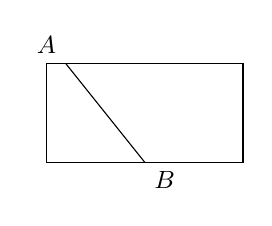
\begin{tikzpicture}[x=5mm,y=5mm,font=\small]
  \draw (0,0) rectangle (5,2.5);
  \draw (.5,2.5)node [above left] () {$A$} -- (2.5,0)node [below right] () {$B$};
\end{tikzpicture}

 \caption{\ref{ese:3.137}}\label{fig:3.6}
 \end{minipage}\hfil
 \begin{minipage}[b]{.20\textwidth}
 \centering % (c) 2012 Dimitrios Vrettos - d.vrettos@gmail.com
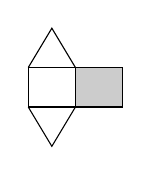
\begin{tikzpicture}[x=6mm,y=5mm]
\fill[gray, opacity=.4](1,0) rectangle (2,1);
\foreach \x in {0,1}
\draw (\x,0) rectangle  (\x+1,1);
\foreach \x in {0}
\foreach \y in {1}{
\draw (\x,\y) -- (\x+.5,\y+1)--(\x+1,\y);
\draw(\x,\y-1)--(\x+.5,-\y)--(\x+1,\y-1);}
\end{tikzpicture}

 \caption{\ref{ese:3.138}}\label{fig:3.7}
 \end{minipage}\hfil
 \begin{minipage}[b]{.20\textwidth}
 \centering% (c) 2012 Dimitrios Vrettos - d.vrettos@gmail.com
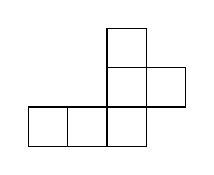
\begin{tikzpicture}[x=5mm,y=5mm]
\foreach \x in {0,1,2}
\draw (\x,0) rectangle (\x+1,1);
\foreach \y in {1,2}
\draw (2,\y) rectangle (3,\y+1);
\draw(3,1) rectangle (4,2);
\end{tikzpicture}

 \caption{\ref{ese:3.139}}\label{fig:3.8}
 \end{minipage}\hfil
 \begin{minipage}[b]{.23\textwidth}
 \centering% (c) 2012 Dimitrios Vrettos - d.vrettos@gmail.com
\begin{tikzpicture}[x=5mm,y=5mm]
\draw (0,0) rectangle (3,3);
\end{tikzpicture}

 \caption{\ref{ese:3.140}}\label{fig:3.9}
 \end{minipage}\hfil
\end{figure}
\end{inaccessibleblock}

\begin{esercizio}
\label{ese:3.137}
Relativamente alla figura~\ref{fig:3.6}, quale proposizione è vera?

\begin{enumeratea}
\item Il segmento~$AB$ la divide in due parti uguali;
\item il segmento~$AB$ la divide in due quadrilateri.
\end{enumeratea}
\end{esercizio}

 \begin{esercizio}
 \label{ese:3.138}
La parte in grigio rappresenta~$1/4$ della figura~\ref{fig:3.7}?
\end{esercizio}

\begin{esercizio}
\label{ese:3.139}
 Costruisci una figura che sia gli~$11/6$ della figura~\ref{fig:3.8}.
\end{esercizio}

\begin{esercizio}
\label{ese:3.140}
Colora i~$3/4$ della figura~\ref{fig:3.9}.
\end{esercizio}
%%%%%%%%%%%%%%%%%%%%%%%%%%%%%%%%%%%%%%

\begin{esercizio}
\label{ese:3.141}
Costruire la frazione~$\frac{N}{D}$ significa dividere l'unità in \ldots 
parti uguali e prendere \ldots parti.
\end{esercizio}

\end{comment}

\begin{esercizio}
\label{ese:3.142}
Rappresenta su una opportuna retta numerica le seguenti frazioni.
\[\frac{3}{4};\quad\frac{3}{8};\quad\frac{1}{3};\quad\frac{5}{4};\quad
\frac{2}{5};\quad\frac{6}{3};\quad\frac{5}{6};\quad%
\frac{12}{4};\quad\frac{19}{8};\quad\frac{16}{5}.\]
\end{esercizio}

\begin{esercizio}[\Ast]
\label{ese:3.143}
Calcola il valore delle seguenti espressioni.
\begin{enumeratea}
\spazielenx
\item $\displaystyle{\bigg(-1+\frac{1}{2}\bigg):\bigg(\frac{3}{2}+
\frac{5}{4}\bigg)}$
  \hfill \(\left[-\dfrac{2}{11} \right]\)
\item $\displaystyle{\bigg(-{\frac{2}{3}}+\frac{1}{2}\bigg)\cdot
\bigg(\frac{1}{2}-\frac{3}{4}\bigg)}$
  \hfill \(\left[\dfrac{1}{24} \right]\)
\item $\displaystyle{\frac{1}{2}\cdot\bigg(-{\frac{1}{4}}+\frac{3}{2}\bigg):
\bigg(\frac{3}{2}-\frac{3}{4}\bigg)}$
  \hfill \(\left[\dfrac{5}{6} \right]\)
\item $\displaystyle{\frac{1}{3}-\bigg(\frac{2}{3}-\frac{5}{6}\bigg)+
\frac{3}{2}-\bigg[\frac{3}{4}-\bigg(\frac{7}{30}%
-\frac{4}{5}\bigg)+\frac{5}{6}\bigg]}$
  \hfill \(\left[-\dfrac{3}{20} \right]\)
\end{enumeratea}
\end{esercizio}

\begin{esercizio}[\Ast]
\label{ese:3.144}
 Calcola il valore delle seguenti espressioni.
\begin{enumeratea}
\spazielenx
\item $\displaystyle{\frac{5}{6}-\frac{2}{3}\cdot\frac{12}{5}+\frac{3}{2}
\cdot\bigg[\frac{3}{4}\cdot%
\bigg(\frac{12}{7}-\frac{5}{2}\bigg)+\frac{5}{6}\bigg]}$
  \hfill \(\left[-\dfrac{673}{1680} \right]\)
\item $\displaystyle{\frac{5}{6}\cdot{\frac{2}{3}}\cdot\frac{12}{5}-
\frac{3}{4}:\bigg[0,75-\frac{5}{6}\bigg]}$
  \hfill \(\left[\dfrac{31}{3} \right]\)
\item $\displaystyle{\frac{1}{3}:\bigg(\frac{3}{2}-\frac{2}{3}\bigg)+
\frac{1}{6}-\frac{1}{15}}$
  \hfill \(\left[\dfrac{1}{2} \right]\)
\item $\displaystyle{-\bigg(\frac{3}{4}+1,4\bigg)\cdot\bigg(\frac{2}{3}-
\frac{3}{8}\bigg)+\frac{6}{5}}$
  \hfill \(\left[\dfrac{55}{96} \right]\)
\end{enumeratea}
\end{esercizio}

\begin{esercizio}[\Ast]
\label{ese:3.145}
 Calcola il valore delle seguenti espressioni.
\begin{enumeratea}
\spazielenx
\item $\displaystyle{\bigg(\frac{2}{3}-\frac{7}{6}\bigg)-\bigg(1+
\frac{5}{6}\bigg):\bigg(2-\frac{1}{3}\bigg)}$
  \hfill \(\left[-\dfrac{8}{5} \right]\)
\item $\displaystyle{\bigg(\frac{5}{3}-\frac{7}{2}\bigg)\cdot\frac{4}{5}+
\bigg[\bigg(\frac{1}{3}-\frac{1}{15}\bigg)%
\cdot\frac{5}{2}\bigg]^{2}}$
  \hfill \(\left[-\dfrac{46}{45} \right]\)
\item $\displaystyle{\frac{63}{55}\cdot\frac{44}{45}+\frac{14}{75}\cdot
\frac{15}{35}+\frac{2}{25}\cdot%
10-\frac{16}{25}:\frac{3}{5}+\frac{1}{15}}$
  \hfill \(\left[1 \right]\)
\item $\displaystyle{\bigg\{\bigg[\bigg(\frac{1}{2}-\frac{2}{3}\bigg):
\bigg(\frac{5}{6}-\frac{5}{12}\bigg)\cdot%
\frac{1}{2}+\frac{3}{4}\bigg]:\frac{1}{4}\bigg\}-\frac{2}{3}\cdot(-0,6)}$
  \hfill \(\left[\dfrac{13}{5} \right]\)
\end{enumeratea}
\end{esercizio}

\begin{esercizio}[\Ast]
\label{ese:3.146}
Calcola il valore delle seguenti espressioni.
\begin{enumeratea}
\spazielenx
\item $\displaystyle{\frac{4}{5}-\frac{27}{7}\cdot{\frac{1}{12}}+
\frac{8}{21}:\frac{8}{6}+\frac{13}{2}\cdot
\frac{1}{7}-\frac{9}{14}+\frac{1}{7}-\frac{12}{25}:\frac{3}{5}}$
  \hfill \(\left[\dfrac{11}{28} \right]\)
\item $\displaystyle{\bigg[\bigg(\frac{1}{3}-\frac{1}{7}\bigg)\cdot
{\frac{7}{2}}-\bigg(\frac{10}{18}-\frac{7}{15}\bigg):\frac{2}{9}\bigg]:
\frac{14}{15}\cdot{\frac{1}{4}}+1}$
  \hfill \(\left[\dfrac{15}{14} \right]\)
\item $\displaystyle{\bigg[\bigg(\frac{4}{3}-\frac{1}{10}\bigg):
\frac{37}{5}+\bigg(\frac{1}{2}\bigg)^{2}-\frac{1}{3}%
\bigg]^{2}:\bigg[\bigg(\frac{1}{2}\bigg)^{2}-\bigg(\frac{1}{3}\bigg)^{2}+
\bigg(\frac{1}{4}\bigg)^{2}-%
\bigg(\frac{1}{6}\bigg)^{2}+\bigg(\frac{5}{12}\bigg)^{2}\bigg]}$
  \hfill \(\left[\dfrac{1}{50} \right]\)
\item $\displaystyle{\bigg(\frac{3}{5}-\frac{1}{4}\bigg)\cdot
\bigg(\frac{7}{5}+\frac{3}{4}\bigg)-\bigg(\frac{2}{3}-%
\frac{5}{4}\cdot\frac{3}{7}\bigg):\frac{2}{14}-\frac{1}{400}}$
  \hfill \(\left[-\dfrac{1}{6} \right]\)
\end{enumeratea}
\end{esercizio}

\begin{esercizio}[\Ast]
\label{ese:3.147}
 Calcola il valore delle seguenti espressioni.
\begin{enumeratea}
\spazielenx
\item $\displaystyle{\bigg(3-\frac{18}{5}-\frac{5}{6}\bigg)\cdot%
\bigg(-{\frac{9}{4}}+\frac{3}{4}\bigg)-\frac{2^{2}}{3}+\frac{1}{60}}$
  \hfill \(\left[\dfrac{5}{6} \right]\)
\item $\displaystyle{\bigg(\frac{3}{5}-1\bigg)-\bigg(\frac{1}{8}+\frac{7}{5}-
\frac{17}{20}\bigg)+%
\bigg(\frac{7}{6}-\frac{2}{5}\bigg):\frac{4}{15}-\bigg(\frac{3}{2}-\frac{5}{2}:
\frac{1}{5}\bigg):\frac{22}{17}-%
\frac{3}{10}}$
  \hfill \(\left[10 \right]\)
\item $\displaystyle{\frac{19}{3}\cdot\bigg(\frac{3}{5}+\frac{3}{2}-2\bigg):
\bigg(\frac{3}{10}-1,25\bigg)-%
\bigg(\frac{1}{2}-\frac{1}{5}-1\bigg)+\frac{3}{2}\cdot\bigg(-{\frac{3}{10}}+
\frac{1}{2}\bigg)\cdot%
\bigg(-{\frac{5}{3}}\bigg)^{2}}$
  \hfill \(\left[\dfrac{13}{15} \right]\)
\item $\displaystyle{\bigg[\bigg(1+\frac{1}{2}\bigg):3-\bigg(2+
\frac{3}{2}\bigg)+1\bigg]+\bigg(3-\frac{3}{4}\bigg)%
+\bigg(\frac{1}{3}+\frac{3}{2}\bigg)-1\bigg(-2+\frac{3}{2}\bigg)^{2}}$
  \hfill \(\left[\dfrac{11}{6} \right]\)
\end{enumeratea}
\end{esercizio}

\begin{esercizio}[\Ast]
\label{ese:3.148}
 Calcola il valore delle seguenti espressioni.
\begin{enumeratea}
\spazielenx
\item $\displaystyle{\bigg[\frac{2}{3}-\bigg(-\frac{1}{4}+\frac{2}{5}\bigg)
\bigg]-\bigg[\frac{3}{5}-%
\bigg(\frac{3}{4}-\frac{1}{3}\bigg)\bigg]}$
  \hfill \(\left[\frac{1}{3} \right]\)
\item $\displaystyle{2-\bigg[3+1-\bigg(2-\frac{1}{2}\bigg)\bigg]-
\bigg(-2-\frac{1}{2}\bigg)\cdot%
\bigg(\frac{1}{2}-\frac{3}{4}+\frac{1}{6}\bigg):\bigg(-{\frac{1}{2}}\bigg)}$
  \hfill \(\left[-\dfrac{1}{12} \right]\)
\item $\displaystyle{\bigg(\frac{8}{3}-\frac{1}{6}\bigg)^{-1}-
\bigg(\frac{1}{2}-\frac{3}{8}\bigg)+\frac{10}{8}\cdot%
\bigg(\frac{5}{7}\bigg)^{-2}+\bigg(\frac{1}{3}\bigg)^{-3}\cdot
\frac{1}{6^{2}}}$
  \hfill \(\left[\dfrac{139}{40} \right]\)
\item $\displaystyle{\bigg\{\bigg(\frac{2}{5}\bigg)^{4}\cdot
\bigg[\bigg(\frac{2}{5}\bigg)^{8}:%
\bigg(\frac{2}{5}\bigg)^{3}\bigg]^{2}\bigg\}^{2}:
\bigg[\bigg(\frac{2}{5}\bigg)^{3}\cdot{\frac{2}{5}}\cdot%
\bigg(\frac{2}{5}\bigg)^{3}\bigg]^{4}}$
  \hfill \(\left[1 \right]\)
\end{enumeratea}
\end{esercizio}

\begin{esercizio}[\Ast]
\label{ese:3.149}
Calcola il valore delle seguenti espressioni.
\begin{enumeratea}
\spazielenx
\item $\displaystyle{1-\bigg[\bigg(\frac{3}{2}\bigg)^{3}\cdot%
\bigg(\frac{3}{2}\bigg)^{2}:\bigg(\frac{3}{2}\bigg)^{4}-
\bigg(\frac{4}{5}\bigg)^{3}:\bigg(\frac{4}{5}\bigg)^{3}+%
\bigg(\frac{1}{3}\bigg)^{4}:\bigg(\frac{1}{3}\bigg)^{3}\bigg]}$
  \hfill \(\left[\dfrac{1}{6} \right]\)
\item $\displaystyle{\bigg(\frac{1}{4}\bigg)^{-2}-\bigg(\frac{1}{2}\bigg)^{-2}+
\frac{2^{2}}{3}\cdot%
\bigg(\frac{2}{3}\bigg)^{-3}-\frac{(-2)^{-2}}{5}-2^{4}}$
  \hfill \(\left[\dfrac{9}{20} \right]\)
\item $\displaystyle{\bigg\{\bigg[\frac{1}{6}+\frac{1}{2}:\bigg(\frac{6}{8}+1-
\frac{3}{4}\bigg)\bigg]^{3}\cdot%
\bigg(\frac{3}{5}-\frac{3}{8}\bigg)+\frac{3}{5}\bigg\}:\frac{1}{5}}$
  \hfill \(\left[\dfrac{10}{3} \right]\)
\item $\displaystyle{\bigg\{\frac{1}{2}+\frac{15}{2}:\bigg[\frac{1}{2}:
\bigg(1-\frac{3}{4}\bigg)+1\bigg]\bigg\}\cdot%
\bigg[\bigg(\frac{1}{3}\bigg)^{5}:\bigg(\frac{1}{3}\bigg)^{4}\bigg]^{2}}$
  \hfill \(\left[\dfrac{1}{3} \right]\)
\end{enumeratea}
\end{esercizio}

\begin{esercizio}[\Ast]
\label{ese:3.150}
 Calcola il valore delle seguenti espressioni.
\begin{enumeratea}
\spazielenx
\item $\displaystyle{\bigg\{\bigg[\bigg(\frac{5}{4}\bigg)^{2}:
\bigg(\frac{1}{2}\bigg)\bigg]\cdot%
\bigg[\bigg(\frac{1}{5}+\frac{1}{10}+\frac{1}{20}\bigg)\cdot\frac{4}{5}\bigg]
\cdot%
\frac{1}{14}\bigg\}^{2}:\bigg(1-\frac{5}{6}\cdot\frac{3}{10}\bigg)^{2}}$
  \hfill \(\left[\dfrac{1}{144} \right]\)
\item $\displaystyle{\bigg[(0,4-1)^{2}:0,01-\bigg(-{\frac{2}{3}}\bigg)^{-2}
\bigg]\cdot
\bigg(-{\frac{1}{2}}\bigg)^{-4}}$
  \hfill \(\left[540 \right]\)
\item $\displaystyle{\frac{7}{23}\bigg\{\bigg(\frac{9}{4}+\frac{3}{4}\cdot
{\frac{1}{2}}-\frac{11}{16}\cdot\frac{1}{2}+\frac{1}{8}\bigg):\bigg[
\bigg(\frac{4}{7}+\frac{5}{4}\bigg):\frac{17}{7}\bigg]\bigg\}\cdot
{\frac{16}{21}}}$
  \hfill \(\left[\dfrac{77}{50} \right]\)
\item $\displaystyle{\bigg(2+\frac{1}{2}\bigg)^{2} \cdot \bigg(2-\frac{1}{2}
\bigg)^{-2}+\bigg[\bigg(2+\frac{1}{3}\bigg)\cdot
\bigg(\frac{7}{3}\bigg)^{-2}\bigg]^{-1}}$
  \hfill \(\left[\dfrac{46}{9} \right]\)
\end{enumeratea}
\end{esercizio}

\begin{esercizio}[\Ast]
\label{ese:3.151}
 Calcola il valore delle seguenti espressioni.
\begin{enumeratea}
\spazielenx
\item $\displaystyle{\bigg[\bigg(3+\frac{1}{2}-\frac{5}{3}\bigg)\cdot
\bigg(\frac{1}{2}\bigg)^{2}\bigg]:\bigg\{\frac{3}{2}-\bigg[\frac{2}{3}+
\bigg(\frac{2}{11}+
\frac{5}{22}+\frac{7}{33}\bigg):\frac{82}{33}+\frac{1}{12}\bigg]^{5}
\bigg\}^{3}:\frac{1}{4}}$
  \hfill \(\left[\dfrac{44}{3} \right]\)
\item $\displaystyle{\bigg\{\bigg[\bigg(\frac{8}{3}\bigg)^{10}:
\bigg(\frac{8}{3}\bigg)^{6}\bigg]^{2}\cdot
\bigg[\bigg(\frac{8}{3}\bigg)^{8}:\bigg(\frac{8}{3}\bigg)^{3}\bigg]\bigg\}:
\bigg(\frac{8}{3}\bigg)^{11}}$
  \hfill \(\left[\dfrac{64}{9} \right]\)
\item $\displaystyle{\bigg(1+\frac{3}{2}\bigg)^{2}\cdot
\bigg(2-\frac{5}{2}\bigg)^{-2}\cdot
\bigg[\bigg(\frac{1}{2}\bigg)^{2}\bigg]^{-2}}$
  \hfill \(\left[400 \right]\)
\item $\displaystyle{\bigg(\frac{1}{3}-1\bigg)-\bigg(\frac{1}{6}-
\frac{1}{4}\bigg)\cdot
{\frac{6}{5}}-\bigg(\frac{2}{9}-\frac{1}{5}\bigg)\cdot 3-\frac{1}{30}}$
  \hfill \(\left[-\dfrac{2}{3} \right]\)
\end{enumeratea}
\end{esercizio}

\begin{esercizio}[\Ast]
\label{ese:3.152}
 Calcola il valore delle seguenti espressioni.
\begin{enumeratea}
\spazielenx
\item $\displaystyle{\cfrac{\bigg(1+\cfrac{2}{3}\bigg):5+\bigg(2-
\cfrac{2}{3}\bigg)}{3+\bigg(\cfrac{1}{2}-1\bigg)}:
\frac{\bigg(5-\cfrac{1}{5}\bigg)+\bigg(\cfrac{7}{3}-\cfrac{2}{35}\bigg)}
{\bigg(\cfrac{3}{2}-\cfrac{1}{4}\bigg)\cdot
\bigg(3-\cfrac{1}{3}\bigg)}}$
  \hfill \(\left[\dfrac{100}{303} \right]\)
\item $\displaystyle{8,75\cdot\bigg(\frac{2}{5}-0,2\bigg)\cdot
\bigg\{\bigg[2-1,\overline{6}-\bigg(0,2+\frac{2}{3}\bigg)\bigg]
\cdot\bigg(\frac{1}{7}-\frac{17}{4}\bigg)\bigg\}-\frac{2}{3}\cdot
\bigg(2-\frac{1}{2}\bigg)+7,5-0,\overline{3}}$
  \hfill \(\left[10 \right]\)
\item $\displaystyle{\bigg[\bigg(\frac{7}{5}-\frac{1}{2}\bigg)^{2}:
\bigg(\frac{9}{10}\bigg)^{2}-
\bigg(1+\frac{2}{3}-2\bigg)^{2}\bigg]^{2}:\bigg(\frac{10}{9}\bigg)^{2}-
\bigg(1+\frac{8}{5}-\frac{1}{25}\bigg)}$
  \hfill \(\left[-2 \right]\)
\item $\displaystyle{\bigg(\frac{1}{6}+0,1\bigg)\cdot 0,16\cdot
(1-1,0\overline{1})^{-1}}$
  \hfill \(\left[-4 \right]\)
\end{enumeratea}
\end{esercizio}

\begin{esercizio}[\Ast]
\label{ese:3.153}
 Calcola il valore delle seguenti espressioni.
\begin{enumeratea}
\spazielenx
\item $\displaystyle{\frac{\bigg\{\bigg[\cfrac{1}{2}-\bigg(2-
\cfrac{11}{4}\bigg)\bigg]:(-3,5)\bigg\}\cdot
\bigg(1-\cfrac{4}{5}\bigg):7^{-2}}{\bigg(-{\cfrac{1}{3}}
\bigg)^{-3}(-3)^{2}(-1)^{2}:(-3)^{2}}}$
  \hfill \(\left[-\dfrac{2}{27} \right]\)
\item $\displaystyle{\bigg(\frac{4}{3}-2\bigg)\bigg(-{\frac{1}{2}}\bigg):
\bigg[\frac{5}{7}\bigg(\frac{2}{5}-\frac{1}{6}\bigg)
+\bigg(2+\frac{2}{5}\bigg)\bigg(\frac{3}{4}-\frac{4}{3}+
\frac{1}{2}\bigg)\bigg]:\frac{11}{6}}$
  \hfill \(\left[-\dfrac{60}{11} \right]\)
\item $\displaystyle{\bigg(1-\frac{1}{2}\bigg)^{-2}\cdot
\bigg[\bigg(1+\frac{1}{2}\bigg)^{2}\bigg]^{-2}:\bigg(\frac{5}{2}-2
\bigg)^{-3}}$
  \hfill \(\left[\dfrac{8}{81} \right]\)
\end{enumeratea}
\end{esercizio}

% \begin{esercizio}[\Ast]
% \label{ese:3.154}
% Calcola il valore della seguente espressione.
% \begin{multline*}
%  \left\{\left[\left(1-\frac{3}{5}\right)^3:\left(\frac{2}{5}\right)^{4}\right]:
%  \left(\frac{2}{5}\right)^{2} \right\}^{6}
% :\left\{\left[\left(\frac{2}{5}\right)^{4}\cdot\left(\frac{7}{5}-
% 1\right)^2\right]^{2}\cdot%
% \left[\left(1-\frac{3}{5}\right)^{5}:\left(\frac{2}{5}\right)^{4}
% \right]^{2}\right\}^{2}
% \end{multline*}
%   \hfill \(\left[\left(\dfrac{2}{5} \right)^{-46} \right]\)
% \end{esercizio}

\begin{esercizio}[\Ast]
\label{ese:3.154}
Calcola il valore della seguente espressione.
\(
\left\{\left[\left(1-\dfrac{3}{5}\right)^3:\left(\dfrac{2}{5}\right)^{4}\right]:
 \left(\dfrac{2}{5}\right)^{2} \right\}^{6}
:\left\{\left[\left(\dfrac{2}{5}\right)^{4}\cdot\left(\dfrac{7}{5}-
1\right)^2\right]^{2}\cdot%
\left[\left(1-\dfrac{3}{5}\right)^{5}:\left(\dfrac{2}{5}\right)^{4}
\right]^{2}\right\}^{2}
\)
  \hfill \(\left[\left(\dfrac{2}{5} \right)^{-46} \right]\)
\end{esercizio}


\begin{esercizio}[\Ast]
\label{ese:3.155}
 Calcola il valore delle seguenti espressioni.
\begin{enumeratea}
\spazielenx
\item $\displaystyle{\bigg(\frac{1}{5}-\frac{1}{4}\bigg)\bigg(-1-
\frac{1}{3}\bigg)+\bigg[\bigg(1+\frac{4}{3}\bigg)\cdot
\bigg(4-\frac{9}{2}\bigg)\bigg]\cdot{\frac{3}{4}}+3-\bigg(\frac{2}{27}
\cdot{\frac{9}{10}}-\frac{1}{10}\bigg)-\frac{9}{40}}$
  \hfill \(\left[2 \right]\)
\item $\displaystyle{\left[0,625+4,5\cdot(0,75-0,\overline{6})\right]:
\left[0,875+0,75\cdot(2,5-2,\overline{3})\right]}$
  \hfill \(\left[1 \right]\)
\item $\displaystyle{\bigg\{3-\bigg[0,\overline{6}-\bigg(0,1\overline{6}+
\frac{5}{12}\bigg)\bigg]:0,25\bigg\}^{2}\cdot
(0,\overline{6}-0,625)}$
  \hfill \(\left[\dfrac{8}{27} \right]\)
\item $\displaystyle{\bigg(\frac{12}{9}-1\bigg)^{2}\cdot\bigg(\frac{2}{81}:3
\bigg)^{-1}\cdot\frac{1}{2}+\bigg(\frac{7}{4}\bigg)^{3}\cdot
\bigg[-\bigg(\frac{4}{3}-\frac{1}{3}\bigg)^{3}\cdot\bigg(\frac{5}{49}-
\frac{3}{147}\bigg)\bigg]-\frac{1}{(-4)^{2}}}$
  \hfill \(\left[\dfrac{25}{4} \right]\)
\end{enumeratea}
\end{esercizio}

\begin{esercizio}[\Ast]
\label{ese:3.156}
 Calcola il valore delle seguenti espressioni.
\begin{enumeratea}
\spazielenx
\item $\displaystyle{\bigg(\frac{1}{5}\bigg)^{2}-\bigg(\frac{1}{6}
\bigg)^{-1}-\frac{\bigg(\frac{1}{3}+0,5\bigg)^{-2}}%
{\bigg(\frac{1}{3}-0,5\bigg)^{-2}}+\bigg(\frac{0,5-0,1}{1-0,5}
\bigg)^{-2}-4^{-2}}$
  \hfill \(\left[-\dfrac{9}{2} \right]\)
\item $\displaystyle{\left[0,1\overline{6}+(0,1\overline{36}+0,41
\overline{6}-0,2\overline{27}):0,3\overline{90}\right]:%
\left[0,\overline{36}+2.25\cdot(0,\overline{5}-0,\overline{27})\right]}$
  \hfill \(\left[1 \right]\)
\item $\displaystyle{\frac{1,6-0,5\cdot(0,\overline{6}-0,5):(1-0,
\overline{6})^{2}-0,7}%
{3\cdot(1-0,5)^{2}+0,875-(1-0,5)^{2}:0,2-0,6\cdot0,5}}$
  \hfill \(\left[2 \right]\)
\item $\displaystyle{{0,1\overline{6}}^{2}+\left[1,5:1,5^{2}+\left(1,
\overline{6}-0,5\right):\left(2-0,\overline{3}\right)%
+\left(0,\overline{6}+0,5-0,2\right)\cdot0,75:5,8\right]\cdot 0,
\overline{6}}$
  \hfill \(\left[\dfrac{38}{45} \right]\)
\end{enumeratea}
\end{esercizio}

\begin{esercizio}[\Ast]
\label{ese:3.157}
 Calcola il valore delle seguenti espressioni.
\begin{enumeratea}
\spazielenx
\item $\displaystyle{\left\{0,8\overline{3}-\left[0,\overline{6}+(0,75-{0,
\overline{6}}^{2}-(1-2,\overline{3}\cdot%
0,25))\right]+0,\overline{6}:0,\overline{8}\right\}:1,02\overline{7}}$
  \hfill \(\left[\dfrac{40}{37} \right]\)
\item $\displaystyle{\frac{1}{\sqrt{3^{2}+4^{2}}}+\frac{1}{\sqrt{13^{2}-12^3}}-
\sqrt{\cfrac{1}{36}+\cfrac{1}{8}%
-\cfrac{1}{24}}}$
  \hfill \(\left[\dfrac{1}{15} \right]\)
\item $\displaystyle{\sqrt{20-2\cdot(2+3)+(2+1)\cdot5}+\sqrt{48:6-3
\cdot2+10:5}}$
  \hfill \(\left[7 \right]\)
\item $\displaystyle{\sqrt{\cfrac{1}{9}\cdot\bigg\{\bigg[\cfrac{11}{3}-
\bigg(\cfrac{1}{3}-\cfrac{1}{4}\bigg)\bigg]:%
\bigg[\bigg(2-\cfrac{7}{4}\bigg)+\cfrac{10}{3}\bigg]\bigg\}}}$
  \hfill \(\left[\dfrac{1}{3} \right]\)
\end{enumeratea}
\end{esercizio}

\begin{esercizio}[\Ast]
\label{ese:3.158}
 Calcola il valore delle seguenti espressioni.
\begin{enumeratea}
\spazielenx
\item $\displaystyle{\sqrt{\bigg\{\bigg[\bigg(\cfrac{5}{4}\bigg)^{2}:
\bigg(\cfrac{1}{4}\bigg)^{2}\bigg]%
\bigg[\bigg(\cfrac{1}{5}+\cfrac{1}{10}+\cfrac{1}{20}\bigg)\cdot\cfrac{4}{5}
\bigg]\cdot\cfrac{1}{4}\bigg\}^{2}%
:\bigg(1-\cfrac{5}{6}\cdot\cfrac{3}{10}\bigg)^{2}}}$
  \hfill \(\left[\dfrac{7}{3} \right]\)
\item $\displaystyle{\left(1+\frac{1}{1-\cfrac{1}{2}}\right)^{-2}\cdot
\left(1-\frac{1}{1+\cfrac{1}{2}}\right)^{2}\cdot%
\bigg(4-\frac{9}{2}\bigg)^{-3}}$
  \hfill \(\left[-\dfrac{8}{81} \right]\)
\end{enumeratea}
\end{esercizio}

% \begin{esercizio}[\Ast]
% \label{ese:3.159}
%  Calcola il valore delle seguenti espressioni.
% \begin{enumeratea}
% \item $\displaystyle{\left[\left(2+\cfrac{1+\cfrac{1}{2}}{1-\cfrac{1}{2}}
% \right)^{-3}\cdot\left(\cfrac{\cfrac{1}{2}-\cfrac{1}{3}}%
% {\cfrac{3}{2}-\cfrac{5}{3}}-\frac{1}{8}\right)\cdot\left(-{\frac{3}{10}}
% \right)^{-2}\right]^{-2}}$
%   \hfill \(\left[100 \right]\)
% \item $\displaystyle{\cfrac{\left[-\left(\cfrac{9}{4}+\cfrac{9}{5}\right)-
% \cfrac{1}{20}\right]\cdot\left(\cfrac{11}{4}-\cfrac{5}{2}\right)}%
% {1-\left[1-\left(-{\cfrac{17}{7}}\right)\right]-\left(-1+\cfrac{2}{7}-
% \cfrac{1}{14}\right)}%
% -\bigg[\bigg(\frac{1}{7}+\frac{33}{21}\bigg)-\bigg(1-\frac{1}{5}-
% \frac{2}{7}\bigg)\bigg]}$
%   \hfill \(\left[-\dfrac{1}{2} \right]\)
% \end{enumeratea}
% \end{esercizio}
% 
% \begin{esercizio}[\Ast]
% \label{ese:3.160}
%  Calcola il valore della seguente espressione.
% \begin{multline*}
% \bigg(\frac{7}{6}-\frac{5}{4}\bigg):\bigg(\frac{1}{12}-\frac{1}{2}\bigg)-
% \frac{3}{10}+\bigg\{\bigg[2-\bigg(2+\frac{1}{2}%
% -\frac{3}{4}+\frac{1}{8}\bigg):\bigg(-{\frac{1}{2}}\bigg)\bigg]\cdot2-
% \frac{7}{10}\bigg\}\\
% \cdot\bigg(-{\frac{2}{3}}+\frac{1}{2}\bigg)%
% +\bigg[\frac{1}{3}+\bigg(1-\frac{1}{4}\bigg):\bigg(-{\frac{9}{2}}\bigg)+
% \frac{1}{15}\bigg].
% \end{multline*}
%   \hfill \(\left[-\dfrac{5}{3} \right]\)
% \end{esercizio}
% 
% \begin{esercizio}[\Ast]
% \label{ese:3.161}
%  Calcola il valore della seguente espressione.
% \begin{multline*}
% \bigg(-{\frac{3}{2}}-1\bigg)\cdot%
% \bigg(-{\frac{3}{2}}+1\bigg)+\bigg(\frac{3}{4}-2\bigg)\cdot%
% \bigg(-{\frac{3}{4}}-2\bigg)\cdot {\frac{4}{11}}+\bigg(\frac{2}{3}-
% \frac{3}{4}\bigg)\\%
% -\bigg[\frac{1}{9}-\bigg(\frac{3}{2}-\frac{2}{3}\bigg):\bigg(\frac{9}{4}+1+%
% \frac{2}{3}-\frac{1}{6}\bigg)+\frac{2}{3}:\bigg(\frac{9}{4}-\frac{9}{4}%
% +\frac{1}{3}\bigg)\bigg]+\bigg(\frac{7}{6}-1\bigg)^{2}.
% \end{multline*}
%   \hfill \(\left[\dfrac{5}{9} \right]\)
% \end{esercizio}
% 
% \begin{esercizio}[\Ast]
% \label{ese:3.162}
%  Calcola il valore della seguente espressione.
% \begin{multline*}
% \bigg[-\bigg(-{\frac{1}{5}}\bigg)^{2}:\bigg(\frac{3}{5}-1\bigg)^{-2}
% \bigg]\cdot%
% \bigg(-1-\frac{1}{5}\bigg)^{-2}\cdot \bigg(-2\bigg)^{-2}\cdot30^{2}\\%
% -\bigg\{-\bigg[\bigg(-3-\frac{1}{4}+\frac{13}{4}\bigg)^{2}:(-4)^{-2}
% \bigg]\bigg\}.
% \end{multline*}
%   \hfill \(\left[-1 \right]\)
% \end{esercizio}
% 
% \begin{esercizio}[\Ast]
% \label{ese:3.163}
%  Calcola il valore della seguente espressione.
% \begin{multline*}
% \bigg[-(-1)^{3}+\bigg(\frac{2}{3}-1\bigg)^{-2}\bigg]\cdot\bigg(-1-\frac{1}{7}
% \bigg)^{-1}\cdot%
% \bigg(\frac{-1}{5}\bigg)^{2}\\%
% +\bigg\{-{\frac{1}{2}}\cdot\bigg[\bigg(-1-\frac{1}{2}\bigg)^{-2}\cdot%
% \bigg(-{\frac{3}{2}}-1\bigg)^{2}\bigg]^{-1}:(-5)^{-2}\bigg\}^{2}.
% \end{multline*}
%   \hfill \(\left[\dfrac{199}{10} \right]\)
% \end{esercizio}
% 
% \begin{esercizio}[\Ast]
% \label{ese:3.164}
%  Calcola il valore della seguente espressione.
% \begin{multline*}
% 1-\bigg(\frac{1}{2}-\frac{3}{4}\bigg)^{2}-\bigg[\frac{3}{4}+
% \bigg(-{\frac{1}{2}}\bigg)^{3}-1+\frac{4}{5}\bigg]:%
% \bigg[-\bigg(\frac{4}{5}\bigg)^{0}-\bigg(\frac{7}{5}-2\bigg)^{2}\bigg]\\%
% -\frac{3}{2}+\bigg[\bigg(-{\frac{4}{5}}\bigg)^{-3}\bigg]^{2}:
% \bigg(-{\frac{4}{5}}\bigg)^{-5}.
% \end{multline*}
%   \hfill \(\left[-\dfrac{3}{2} \right]\)
% \end{esercizio}

\begin{esercizio}
\label{ese:3.165}
Calcola il valore dell'espressione~$E = A- B$, dove
\[A=\left(\left(\left(-{\frac{3}{7}}\right)^{4}:
\left(-{\frac{7}{3}}\right)^{-2}\right)\cdot%
\left(\frac{3}{7}\right)^{-1}\right)^{-2},\qquad
B=\left(\left(\frac{3}{7}\right)^{-6}\cdot%
\left(1-\frac{4}{7}\right)^{5}\right)^{2}.\]
 \end{esercizio}

 \begin{multicols}{2}
% \begin{esercizio}[\Ast]
% \label{ese:3.166}
%  L'età di Paolo è i~$5/11$ di quella della madre che ha~44 anni. 
%  Quanti anni ha Paolo? \hfill [20]
% \end{esercizio}
% 
% \begin{esercizio}[\Ast]
% \label{ese:3.167}
% L'età di Marco è~$1/2$ di quella di Paolo che è~$1/3$ di quella del padre che 
% ha~54 anni. Quanti anni ha Marco? \hfill [9]
% \end{esercizio}
% 
% \begin{esercizio}[\Ast]
% \label{ese:3.168}
% I~$2/5$ del libro che stiamo leggendo è la parte più noiosa. Le rimanenti~63 
% pagine sono invece le più avvincenti.
% Di quante pagine è formato il libro? \hfill [105]
% \end{esercizio}

% \begin{esercizio}[\Ast]
% \label{ese:3.169}
% Gli alunni del primo e del secondo anno di una scuola media sono 
% rispettivamente i~$3/7$ e i~$2/7$ del totale.
% Sapendo che gli alunni che frequentano la terza media sono~54, quanti sono 
% tutti gli alunni della scuola? \hfill [189]
% \end{esercizio}
% 
% \begin{esercizio}[\Ast]
% \label{ese:3.170}
% Al supermercato ho speso~$7/10$ della somma di denaro che possedevo;
% successivamente ho incassato un credito uguale ai~$13/20$ della somma
% iniziale e ho speso~$2/15$ sempre della somma iniziale per un
% rifornimento di benzina. Sapendo che sono rimasto con~220,50 euro,
% quale somma di denaro possedevo inizialmente? \hfill [270]
% \end{esercizio}
% 
% \begin{esercizio}[\Ast]
% \label{ese:3.171}
%  In una fattoria ci sono vitelli, capre e animali da cortile per
% un totale di~75 capi. I vitelli sono i~$2/5$ di tutti gli animali,
% mentre le capre sono i~$2/3$ degli animali da cortile. Quanti vitelli,
% capre e animali da cortile ci sono? \hfill [30,~18,~27]
% \end{esercizio}
% 
% \begin{esercizio}[\Ast]
% \label{ese:3.172}
%  Tre casse pesano complessivamente~$220\unit{kg}$ la seconda pesa~$1/2$ della
% prima e la terza pesa~$1/3$ della seconda. Calcola il peso di ciascuna
% cassa. \hfill [132,~66,~22]
% 
% \end{esercizio}
% 
% \begin{esercizio}[\Ast]
%  \label{ese:3.173}
% Tre operai devono eseguire un lavoro. Il primo da solo lo farebbe in
% 12 giorni, il secondo in~18 giorni e il terzo in~36 giorni. Lavorando
% insieme, in quanti giorni i tre operai potrebbero eseguire tutto il
% lavoro? \hfill [6]
% \end{esercizio}
% 
% \begin{esercizio}[\Ast]
% \label{ese:3.174}
%  Un collezionista vende i~3/7 della sua collezione costituita da~385
% pezzi. Quanti pezzi gli rimangono? \hfill [220]
% \end{esercizio}

% \begin{esercizio}[\Ast]
% \label{ese:3.175}
%  In un terreno agricolo sono stati piantati ulivi e mandorli per~266
% alberi complessivi. Se gli ulivi sono i~4/10 degli alberi di mandorle,
% quanti sono gli ulivi e i mandorli \hfill [76,~190]
% \end{esercizio}
% 
% \begin{esercizio}[\Ast]
% \label{ese:3.176}
% Il prezzo di copertina di un libro è di~29 euro; quanto verrà
% pagato con uno sconto del~15\%? \hfill [\officialeuro\ 24,65]
% \end{esercizio}
% 
% \begin{esercizio}[\Ast]
% \label{ese:3.177}
% Su~1020 alunni di una scuola,~153 sono stati respinti; qual è la
% percentuale dei promossi? \hfill [85]
% \end{esercizio}
% 
% \begin{esercizio}[\Ast]
% \label{ese:3.178}
%  La differenza di età fra Marco e Antonio è di~18 anni e
% l'età di Marco è i~7/4 di quella di Antonio. Quanti
% anni hanno Marco e Antonio? \hfill [42,~24]
% \end{esercizio}

\begin{esercizio}
\label{ese:3.179}
 Un oggetto è costituito da una lega di zinco e rame. Il suo peso
è di~$280\unit{g}$ e la percentuale di rame è il~20\%. Quanti grammi di zinco
contiene? \hfill [\dots]
\end{esercizio}

% \begin{esercizio}[\Ast]
% \label{ese:3.180}
%  Mario va in pizzeria e, nell'attesa di essere
% servito, conta le persone che vi si trovano: gli uomini sono i~5/9
% delle donne, queste superano gli uomini di~8 unità, infine vi sono~17
% bambini. Quante persone ci sono in tutto? Quanti sono gli uomini e le
% donne? \hfill [45,~10,~18]
% \end{esercizio}
% 
% \begin{esercizio}[\Ast]
% \label{ese:3.181}
%  Gino compra un'auto da~5\,400 euro. Paga i~4/9 in contanti ed il resto
% in~5 rate. Qual è l'ammontare di ogni rata? A quale
% frazione corrisponde ogni rata? \hfill [\officialeuro\ 600,~1/9]
% \end{esercizio}
% 
% \begin{esercizio}[\Ast]
% \label{ese:3.182}
%  Il serbatoio di una macchina contiene benzina per i~3/4 della sua
% capacità. Dopo aver consumato i~2/3 della benzina che
% c'è, si fa un pieno aggiungendone~66 litri. Qual è
% la capacità del serbatoio? \hfill [88]
% \end{esercizio}

\begin{esercizio}
\label{ese:3.183}
 Un misurino contiene~1/8 di kg di farina. Quanti misurini di farina
sono necessari per riempire un sacchetto di~$5\unit{kg}$? \hfill [\dots]
\end{esercizio}

% \begin{esercizio}[\Ast]
% \label{ese:3.184}
%  Due gruppi di scavatori scavano una galleria, ciascun gruppo comincia
% da una delle due parti opposte; se fino a oggi hanno scavato
% rispettivamente~5/9 e~3/7 dell'intera galleria e
% restano ancora da scavare~$2\unit{m}$, quanto è lunga
% l'intera galleria? \hfill [126]
% \end{esercizio}
% 
% \begin{esercizio}[\Ast]
% \label{ese:3.185}
%  L'aria è composta per~39/50 di azoto e per~21/100 di
% ossigeno, la parte rimanente è composta da gas diversi. Quale
% frazione di aria occupano tutti gli altri gas? \hfill [1/100]
% \end{esercizio}
% 
% \begin{esercizio}[\Ast]
% \label{ese:3.186}
%  Luca ha pagato la tassa scolastica in ritardo, ha pagato \officialeuro\ 56,16
% compresa la mora del~4\% per il ritardo nel pagamento.
% Quanto avrebbe dovuto pagare senza mora? \hfill [\officialeuro\ 54]
% \end{esercizio}

\begin{esercizio}
\label{ese:3.187}
 In un'azienda~3/10 degli impiegati sono addetti
contabilità. Qual è la percentuale degli addetti contabilità
rispetto a tutti gli impiegati azienda? \hfill [\dots]
\end{esercizio}

\begin{esercizio}
\label{ese:3.188}
 A un gruppo di~200 intervistati è stato chiesto quale quotidiano
leggono. Le risposte sono state le seguenti:
\begin{itemize*}
\item 90 leggono ``La Repubblica'';
\item 70 leggono ``Il Corriere della sera'';
\item 30 leggono ``La stampa'';
\item 10 leggono ``La gazzetta dello sport''.
\end{itemize*}
Trasforma in percentuali i dati ottenuti. \hfill [\dots]
\end{esercizio}

\begin{esercizio}
\label{ese:3.189}
 A un concorso si sono presentati~324 candidati.~22 hanno superato il
concorso. Qual è stata la percentuale dei candidati che non hanno
superato il concorso? \hfill [\dots]
\end{esercizio}

% \begin{esercizio}[\Ast]
% \label{ese:3.190}
% Un'auto usata è stata acquistata a \officialeuro\ 11\,800
% in questo modo: il~5\% come caparra per la prenotazione, il
% 20\% al momento della consegna e il resto in~12 rate di pari importo.
% Qual è l'importo della rata? \hfill [\officialeuro\ 737,50]
% \end{esercizio}
% 
% \begin{esercizio}[\Ast]
% \label{ese:3.191}
% Un gestore di un bar acquista i cornetti a \officialeuro\ 0,60 rivende a
% \officialeuro\ 0,75. Qual è la percentuale di guadagno sul prezzo di
% acquisto? \hfill [25\%]
% \end{esercizio}

\begin{esercizio}
\label{ese:3.192}
In un supermercato si vende il pomodoro pelato a \officialeuro\ 0,60 in
confezioni da~$250\unit{g}$ e a~1,00 euro in confezioni da~$500\unit{g}$ 
Qual è la percentuale di sconto che usufruisce chi compra la confezione da 
mezzo chilo? \hfill [\dots]
\end{esercizio}

% \begin{esercizio}[\Ast]
% \label{ese:3.193}
% In una piscina contenente~$2800\unit{m\textsuperscript{3}}$ di acqua si devono
% aggiungere~15 litri di cloro. Quanto cloro occorre per
% $1000\unit{m\textsuperscript{3}}$ di acqua? \hfill [$5,36\unit{l}$]
% \end{esercizio}

% \begin{esercizio}[\Ast]
% \label{ese:3.194}
% La somma di due segmenti misura~$34\unit{cm}$, sapendo che le loro lunghezze
% sono in proporzione con~3/2, calcola la loro lunghezza. 
% \hfill [$13,6\unit{cm}$,~$20,4\unit{cm}$]
% \end{esercizio}
% 
% \begin{esercizio}[\Ast]
% \label{ese:3.195}
% Gli angoli interni di un triangolo hanno misure proporzionali ai
% numeri~1;~3;~5. Ricordando che la somma degli angoli interni di un
% triangolo misura~180{\textdegree}, calcola le misure degli angoli. 
% \hfill [20{\textdegree},~60{\textdegree},~100{\textdegree}]
% \end{esercizio}

\begin{esercizio}
\label{ese:3.196}
Un televisore a~16/9 ha la base di~18 pollici. Quanti
pollici misura l'altezza? \hfill [\dots]
\end{esercizio}

\begin{esercizio}
\label{ese:3.197}
Per preparare una torta bisogna mettere~3 parti di zucchero ogni~4
parti di farina. Se si utilizzano~500g di farina, quanto zucchero
bisogna utilizzare? \hfill [\dots]
\end{esercizio}

% \begin{esercizio}[\Ast]
% \label{ese:3.198}
% Un negoziante, durante il periodo di Natale, aumenta tutti i prezzi del
% 10\%. Se il prezzo iniziale di un paio di scarpe era \officialeuro\ 70,00
% qual è ora il suo prezzo? Dopo le feste, il negoziante abbassa i
% nuovi i prezzi del~10\%. Quanto costano ora le
% scarpe? \hfill [\officialeuro\ 77; \officialeuro\ 69,30]
% \end{esercizio}

% \begin{esercizio}[\Ast]
% \label{ese:3.199}
% Al cinema ``Pegaso'' hanno deciso di aumentare il biglietto del~10\%; 
% il numero degli spettatori
% è calato, però, del~10\%. È stato un affare? Spiega perché. 
% \hfill [No, perde l'1\% dei ricavi]
% \end{esercizio}

\begin{esercizio}
\label{ese:3.201}
 Anna entra in una cartoleria e compra due penne, di cui una costa il
doppio dell'altra; riceve lo sconto~15\% sulla penna
più costosa e del~40\% su quella meno costosa. Qual è lo sconto che
riceve complessivamente? \hfill [21\%]
\end{esercizio}

% \begin{esercizio}[\Ast]
% \label{ese:3.202}
% Pierino oggi ha incrementato il suo capitale del~10\%. Se anche
% domani l'incremento sarà del~10\%, quanto sarà
% l'incremento totale in percentuale? \hfill [\dots]
% \end{esercizio}
% 
% \begin{esercizio}
% \label{ese:3.203}
% Tizio ha perso il~20\% dei suoi soldi; quanto dovrà guadagnare, in
% percentuale, per recuperare? \hfill [\officialeuro\ 50]
% \end{esercizio}
% 
% \begin{esercizio}[\Ast]
% \label{ese:3.204}
% Un paio di scarpe scontato del~20\% costa \officialeuro\ 40 quanto
% costava prima dello sconto? \hfill [\dots]
% \end{esercizio}

\begin{esercizio}
\label{ese:3.205}
Per pavimentare una piazza~8 operai impiegano~10 giorni
lavorando~8 ore al giorno; quanti giorni impiegherebbero~5 operai se
lavorassero~6 ore al giorno? \hfill [\dots]
\end{esercizio}

\begin{esercizio}
\label{ese:3.206}
Pierino si reca in un negozio di giocattoli, dove ne acquista uno. A
Pierino vengono offerti due tipi di sconti, uno del~10\% e uno del
35\%. In quale ordine converrà ricevere i due sconti? Spiega il
motivo. \hfill [\officialeuro\ 2,15]
\end{esercizio}

% \begin{esercizio}[\Ast]
% \label{ese:3.207}
% Una tariffa telefonica ha un costo di~10 cent al minuto per i primi~5
% minuti di conversazione. Per i minuti successivi aumenta del~5\%. Dopo
% 15 minuti di conversazione aumenta del~20\% del costo iniziale. Quanto
% si spende se si effettua una telefonata di~20 minuti? \hfill [\dots]
% \end{esercizio}

\begin{esercizio}
\label{ese:3.208}
Un ingegnere incassa per la realizzazione di un progetto una
certa somma. Di essa il~20\% deve essere restituita allo stato come IVA
e della parte rimanente il~40\% deve essere pagata come tasse. Qual è
la percentuale della somma che rimane all'ingegnere? \hfill [\dots]
\end{esercizio}

\begin{esercizio}
\label{ese:3.209}
Nel paese di Vattelapesca il~20\% degli abitanti è europeo il
restante~80\% è asiatico. La lingua inglese è parlata dal~50\% degli
europei e dal~40\% degli asiatici. Se a Vattelapesca~5\,930 persone
parlano inglese, quanti sono gli abitanti di Vattelapesca? \hfill [\dots]
\end{esercizio}

\begin{esercizio}
\label{ese:3.210}
Un liquido viene filtrato con un primo filtro che toglie il~40\%
delle impurità. Successivamente viene filtrato con un secondo filtro
che toglie il~30\% delle impurità. Infine viene filtrato con un terzo
filtro che elimina il~50\% delle impurità. Quale percentuale
complessiva delle impurità è stata eliminata? \hfill [\dots]
\end{esercizio}

\begin{esercizio}
\label{ese:3.211}
Una prova di ammissione consiste di due test. Solo i~2/3 dei
candidati superano il primo test e~1/5 di quelli che hanno superato il
primo test superano anche il secondo. Qual è la percentuale di
candidati che hanno superato tutti e due i test? \hfill [\dots]
\end{esercizio}

\begin{esercizio}
\label{ese:3.212}
L'acquisto di un'auto può essere fatto con due tipi di pagamento: pagando
l'intero importo di \officialeuro\ 23\,000 all'acquisto il~1{\textdegree} 
gennaio~2011; oppure
dividendo il pagamento in tre rate annuali di~8000, da pagare il
1{\textdegree} gennaio~2011, il~1{\textdegree} gennaio~2012, il
1{\textdegree} gennaio~2013. Avendo tutto il denaro su un conto
corrente bancario a un interesse annuo del~3\% quale forma di pagamento
è più vantaggiosa? Di quanto? \hfill [\dots]
\end{esercizio}

\begin{esercizio}
\label{ese:3.213}
Una forte influenza ha colpito il~60\% dei bambini di età
inferiore o uguale a~10 anni e il~15\% delle persone di età maggiore.
Se la percentuale di persone che si sono ammalate di questa influenza
è stata del~20\%, qual è la percentuale di bambini in quella
popolazione? \hfill [19,19\%]
\end{esercizio}

% \begin{esercizio}[\Ast]
% \label{ese:3.214}
%  Una maglietta costava lire~65.000 prima
% dell'entrata in vigore dell'euro, dopo costava €~40. Di
% quanto è aumentato in \%, il prezzo della maglietta? Si
% tenga conto che~1 \officialeuro\ valeva~1936,77 lire. \hfill [\dots]
% \end{esercizio}

\begin{esercizio}
\label{ese:3.215}
 Una ragazza, di~$46\unit{kg}$, va dal dietologo, che
le consiglia di restare entro il~5\% del peso attuale. Tra
quali valori può oscillare il suo peso? \hfill [\dots]
\end{esercizio}

\begin{esercizio}
\label{ese:3.216}
Per raccogliere le foglie cadute nel cortile
della scuola, Mario impiega~6 ore, Marco~10 ore,
Matteo~15 ore. Se i tre si mettessero a lavorare
insieme, in quante ore pulirebbero il cortile? \hfill [\dots]
\end{esercizio}
% 
% \begin{esercizio}
% \label{ese:3.217}
% Una certa bevanda è ottenuta mescolando~1
% parte di sciropppo con~5 parti di acqua. Per errore
% Adolfo ha mescolato~5 parti di sciroppo con~1 di
% acqua, ottenendo~3 litri di miscuglio. Aggiungendo
% una opportuna quantità di acqua, Adolfo può ottenere
% una bevanda in cui sono rispettate le proporziioni
% stabilite? Quanti litri di acqua deve aggiungere? \hfill [\dots]
% \end{esercizio}
\end{multicols}
